\documentclass[a4paper, 12pt]{article}

\usepackage{enumerate}
\usepackage{hyperref}
\hypersetup{
	colorlinks=true,
	linkcolor=blue,
	filecolor=blue,
	urlcolor=blue,
	citecolor=blue,
}
\usepackage{amsmath}
\usepackage{amsthm}
\usepackage{amssymb}
\usepackage[margin=3cm]{geometry}
\usepackage{mathpazo}
\usepackage{url}
\usepackage{subcaption}
\usepackage{tikz}
\usepackage{pgf}
\usepackage{longtable}
\usepackage{multirow}
\usepackage{graphicx}
\usepackage{pgfplots}
\usepackage{cleveref}
\usepackage{amsrefs}
\usepackage{bbm}
\usepackage{csquotes}
\usepackage{wrapfig}
\usepackage{algorithm}
\usepackage{algpseudocode}
\usepackage{mathrsfs}
\usepackage{afterpage}

\numberwithin{equation}{section}
\numberwithin{figure}{section}

\newtheorem{thm}{Theorem}[section]
\newtheorem*{thm*}{Theorem}
\newtheorem*{con*}{Conjecture}
\newtheorem{lem}[thm]{Lemma}
\newtheorem{prop}[thm]{Proposition}
\newtheorem{cor}[thm]{Corollary}
\newtheorem{lemma}[thm]{Lemma}
\newtheorem{conj}[thm]{Conjecture}

\theoremstyle{definition}
\newtheorem{defn}[thm]{Definition}
\newtheorem{remark}[thm]{Remark}
\newtheorem{ex}[thm]{Example}
\newtheorem{quest}[thm]{Question}
\newtheorem{obs}[thm]{Observation}

\renewcommand{\leq}{\leqslant}
\renewcommand{\geq}{\geqslant}
\newcommand{\N}{\mathbb{N}}
\newcommand{\Z}{\mathbb{Z}}
\newcommand{\Q}{\mathbb{Q}}
\newcommand{\R}{\mathbb{R}}
\newcommand{\C}{\mathbb{C}}
\newcommand{\tr}{\mathrm{t}}
\newcommand{\WEEK}[1]{%
\hfill Week #1

\vspace{-1em}

\begin{center}
	\rule{\textwidth}{2pt}
\end{center}
\vspace{0.5em}%
}

\renewcommand{\algorithmicrequire}{\textbf{Input:}}
\renewcommand{\algorithmicensure}{\textbf{Output:}}

% Configure comments to flush right
\renewcommand{\algorithmiccomment}[1]{\hfill \# #1}

\setcounter{tocdepth}{2}

\allowdisplaybreaks

\title{Geometric Foundations of Data Analysis I}
\author{Joshua Maglione}
\date{\today}

\begin{document}

\maketitle
\tableofcontents

\section{Introduction}

Data analysis and more broadly Data Science is a vast and important field within
Computer Science and Mathematics. At the core, the goal is to make sense of
data, which can be measurements, survey results, behavior patterns, etc. Often
this data comes to us in a very ``high dimension''. That is, there are so many
variables that it is impossible to visualize, and even in low
dimensions, it may not be clear what the best conclusion is based on the
analysis. 

A few references seem to agree that the \textit{total data} on all computers is
something like $\mathbf{10^{23}}$ \textbf{bytes} or about \textbf{100
zettabytes}. While all of this data is not concentrated in one organization, we
still require highly sophisticated tools to make sense of a huge amount of data.
My goal with this course is that you will have a solid foundation with some
standard tools. From this bedrock one could explore more sophisticated methods
of data analysis more easily. 

\bigskip

\noindent We will consider four key topics:
\begin{enumerate} 
	\item Least Squares Fitting,
	\item Principal Component Analysis,
	\item $k$-Means and Hierarchical Clustering,
	\item Nearest Neighbors and the Johnson--Lindenstrauss Theorem
\end{enumerate}

We will be working with the assumption that \textbf{the data we care about is
preserved by orthogonal and linear transformations}. This is not true with all
data---for example, one should not take (proper) linear combinations of people.
However, for data like grams of different kinds of food, this is completely
plausible. This assumption will not always be necessary, but we will just keep
this in mind. 

Half of our time will be spent bringing these ideas to life and getting our
hands dirty. We will be working with Jupyter Notebooks to build familiarity with
the concepts we will discuss. This will be done using Python and standard data
analysis packages like Pandas. 

\section{Least squares fitting}

This method of analysis is both simple and powerful. Like with most things in
mathematics, without some good guiding examples, we can get lost in the
formulas.

\subsection{Build up}\label{sec:build-up}

Suppose we have the following data as seen in \Cref{fig:2d-linear-data}. (Maybe
a company produces parts once per month in lots that vary in size depending on
demand. We write $i$ for the production run, $x_i$ for the lot size, and $y_i$
for the hours of labor.) 

\begin{figure}[h]
	\centering
	\begin{minipage}{0.33\textwidth}
		\centering
		\begin{tabular}{ccc}
			$i$ & $x_i$ & $y_i$ \\ \hline 
			1 & 30 & 73 \\ 
			2 & 20 & 50 \\
			3 & 60 & 128 \\
			4 & 80 & 170 \\
			5 & 40 & 87 \\
			6 & 50 & 108 \\
			7 & 60 & 135 \\
			8 & 30 & 69 \\
			9 & 70 & 148 \\
			10 & 60 & 132 
		\end{tabular}
	\end{minipage}~%
	\begin{minipage}{0.60\textwidth}
		\centering
		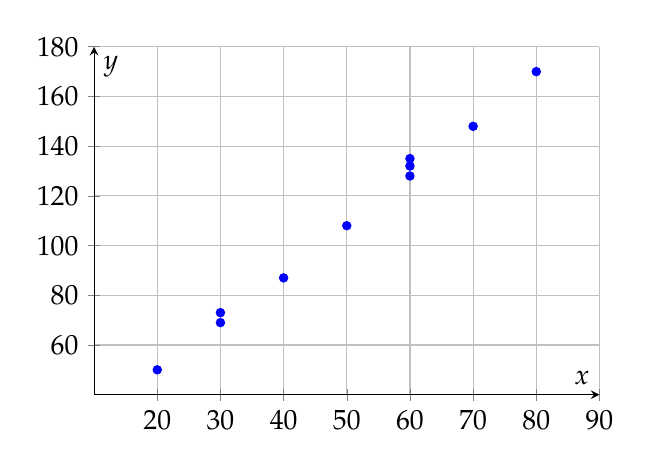
\begin{tikzpicture}
			\begin{axis}[
				xlabel={$x$},
				ylabel={$y$},
				xmin=10, xmax=90,
				ymin=40, ymax=180,
				xtick={10,20,...,90},
				ytick={40,60,...,180},
				grid=both,
				axis lines=middle,
				width=8cm,
				height=6cm,
				]
				\addplot[only marks, mark=*, mark size=1.5pt, color=blue] table {
				30 73
				20 50
				60 128
				80 170
				40 87
				50 108
				60 135
				30 69
				70 148
				60 132
				};
			\end{axis}
		\end{tikzpicture}
	\end{minipage}
	\caption{Data points exhibiting a linear relationship.}
	\label{fig:2d-linear-data}
\end{figure}

It seems clear from the plot that the data fits a geometric pattern---there is a
linear phenomenon. If we try to find the line that is somehow closest to all the
data points, we might draw something like in \Cref{fig:2d-linear-data-line}. 

\begin{figure}[h] 
	\centering
	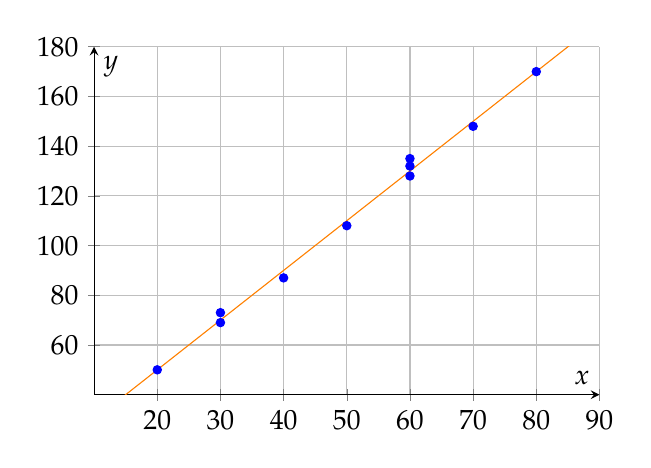
\begin{tikzpicture}
		\begin{axis}[
			xlabel={$x$},
			ylabel={$y$},
			xmin=10, xmax=90,
			ymin=40, ymax=180,
			xtick={10,20,...,90},
			ytick={40,60,...,180},
			grid=both,
			axis lines=middle,
			width=8cm,
			height=6cm,
			]
			\addplot[only marks, mark=*, mark size=1.5pt, color=blue] table {
			30 73
			20 50
			60 128
			80 170
			40 87
			50 108
			60 135
			30 69
			70 148
			60 132
			};
			\addplot[domain=0:90, samples=2, color=orange]{10 + 2*x};
		\end{axis}
	\end{tikzpicture}
	\caption{Line of best fit with data points.}
	\label{fig:2d-linear-data-line}
\end{figure}

Although the line is not a perfect fit, it seems to tell us something about the
relationship between the lots size and the amount of hours. 

\textbf{Questions:}
\begin{itemize}
	\item What makes this line ``better'' than alternatives?
	\item How are we quantifying ``better''? 
	\item Why are we using a line? 
\end{itemize}
We will answer the first question later, probably. Let us consider the question
of quantifying ``better''. Least squares fitting is all about minimizing the
squares of differences between the line and the actual data points. We will make
this precise very soon.

\subsection{Line of best fit}

We know that the equation of a non-vertical line has the form 
\begin{align*}
	y &= b_0 + b_1x.
\end{align*}
If we had $n$ data points of the form $(x_i,y_i)$, we could choose $b_0$ and
$b_1$ to minimize the following sum
\begin{align*}
	S(b_0,b_1) = \sum_{i=1}^n \left(y_i - (b_0 + b_1x_i)\right)^2 .
\end{align*}

We can even solve for these values. Since $S$ is a function in terms of $b_0$
and $b_1$, all possible minima occur when the partial derivatives of $S$ are
$0$. In other words, the minima arise as values $(b_0,b_1)$ such that 
\begin{align*}
	\dfrac{\partial S}{\partial b_0} &= -2\sum_{i=1}^n \left(y_i - (b_0 + b_1x_i)\right) = 0, \\
	\dfrac{\partial S}{\partial b_1} &= -2\sum_{i=1}^n \left(x_iy_i - x_i(b_0 + b_1x_i)\right) = 0.
\end{align*}
These equations are linear equations, so we can solve for these with techniques
from linear algebra. This mean, we need to solve two equations in the unknown
$b_0$ and $b_1$:
\begin{equation}\label{eqn:least-squares-line}
	\begin{split}
		nb_0 + b_1\sum x_i &= \sum y_i, \\
		b_0 \sum x_i + b_1 \sum x_i^2 &= \sum x_iy_i. 
	\end{split}
\end{equation}

Using the data from our example in \Cref{sec:build-up}, we have 
\begin{align*}
	\sum x_i &= 500, & 
	\sum y_i &= 1100, & 
	\sum x_i^2 &= 28400, & 
	\sum x_iy_i &= 61800. 
\end{align*}
Thus, the equations we need to solve are 
\begin{align*}
	10b_0 + 500b_1 &= 1100, \\
	500b_0 + 28400b_1 &= 61800,
\end{align*}
which yield $b_0=10$ and $b_1 = 2$. Going back to the context of the initial
problem: this solution tells us that by increasing the lot size by one, we
expect to increase the labor hours by two. 

\subsubsection{Written as matrices}

Let us write the equations in~\eqref{eqn:least-squares-line} with matrices. This
might seem like overkill at this stage, but it will set us up nicely to
generalize. Let 
\begin{align}\label{eqn:X-Y-B}
	X &= \begin{pmatrix}
		1 & x_1 \\
		1 & x_2 \\
		\vdots & \vdots \\
		1 & x_n
	\end{pmatrix}, & 
	Y &= \begin{pmatrix}
		y_1 \\ y_2 \\ \vdots \\ y_n
	\end{pmatrix}, & 
	B &= \begin{pmatrix}
		b_0 \\ b_1 
	\end{pmatrix}. 
\end{align}
Therefore, the equations in~\eqref{eqn:least-squares-line} are equivalent to the
single matrix equation:
\begin{align}
	X^\tr XB = X^\tr Y.
\end{align}
If $X^{\tr} X$ is invertible, then $B = (X^{\tr}X)^{-1}X^{\tr}Y$.

\subsection{In class exercises pt. I}

\begin{enumerate}
	\item 
	\begin{enumerate} 
		\item With $X$, $Y$, and $B$ as defined in \Cref{eqn:X-Y-B}, show that 
		\begin{align*}
			X^\tr X &= \begin{pmatrix}
				n & \sum x_i \\ \sum x_i & \sum x_i^2
			\end{pmatrix}, & 
			X^\tr Y &= \begin{pmatrix}
				\sum y_i \\ \sum x_iy_i
			\end{pmatrix}. 
		\end{align*}
		\item Show that $X^\tr XB = X^\tr Y$ is equivalent to
		\Cref{eqn:least-squares-line}:
		\begin{align*}
			nb_0 + b_1\sum x_i &= \sum y_i, \\
			b_0 \sum x_i + b_1 \sum x_i^2 &= \sum x_iy_i.
		\end{align*}
	\end{enumerate}
	\item Find a least squares fitting line to the following data and draw in
	the line:
	
	\begin{minipage}{0.3\textwidth}
		\centering 
		\begin{tabular}{ccc}
			$i$ & $x_i$ & $y_i$ \\ \hline
			1 & 1.0 & 1.0 \\ 
			2 & 2.0 & 1.5 \\
			3 & 3.0 & 2.0 \\
			4 & 1.5 & 2.0 \\ 
			5 & 3.5 & 3.0 \\ 
			6 & 3.0 & 4.5 \\ 
			7 & 4.0 & 2.0 \\ 
			8 & 5.0 & 3.5
		\end{tabular}
	\end{minipage}~%
	\begin{minipage}{0.6\textwidth}
		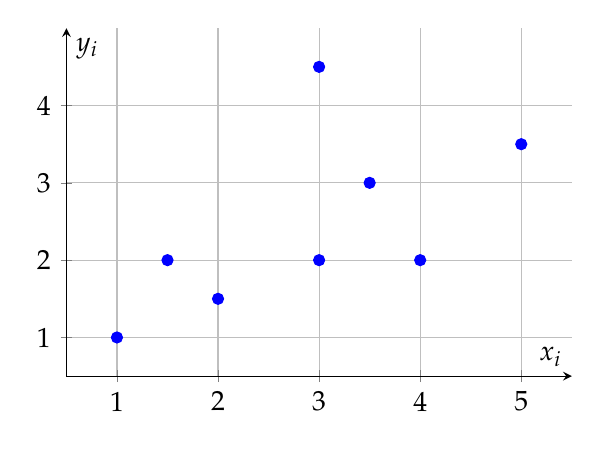
\begin{tikzpicture}
			\begin{axis}[
				xmin=0.5, xmax=5.5,
				ymin=0.5, ymax=5,
				xlabel={$x_i$},
				ylabel={$y_i$},
				xtick={1,2,3,4,5},
				ytick={1,2,3,4},
				grid=both,
				axis lines=middle,
				width=8cm,
				height=6cm,
			]
			\addplot[only marks, mark=*, mark size=2pt, color=blue] table {
				1.0 1.0
				2.0 1.5
				3.0 2.0
				1.5 2.0
				3.5 3.0
				3.0 4.5
				4.0 2.0
				5.0 3.5
			};
			% \addplot[domain=0:90, samples=2, color=orange]{0.94 + 0.52*x};
			\end{axis}
		\end{tikzpicture}
	\end{minipage}

	(Round $b_0$ and $b_1$ to the nearest half integer.)
\end{enumerate}

\WEEK{1}


\subsection{Plane of best fit}

We consider two independent variables and one dependent variable now. Consider
the following data points as given in \Cref{fig:3d-data-points}.

\begin{figure}[h]
	\centering
	\begin{minipage}{0.3\textwidth}
		\centering 
		\begin{tabular}{cccc}
			$i$ & $x_{i1}$ & $x_{i2}$ & $y_i$ \\ \hline
			0 & 278 & 36 & 287 \\
			1 & 252 & 31 & 256 \\
			2 & 344 & 35 & 300 \\
			3 & 134 & 33 & 182 \\
			4 & 215 & 35 & 248 \\
			5 & 261 & 40 & 271 \\
			6 & 131 & 39 & 149 \\
			7 & 463 & 43 & 411 \\
			8 & 167 & 46 & 214 \\
			9 & 298 & 42 & 291 \\
			10 & 230 & 60 & 314 \\
			11 & 293 & 67 & 352 \\
			12 & 290 & 37 & 298 \\
			13 & 271 & 31 & 252 \\
			14 & 385 & 63 & 439 \\
			15 & 354 & 36 & 328
		\end{tabular}
	\end{minipage}~%
	\begin{minipage}{0.6\textwidth}
		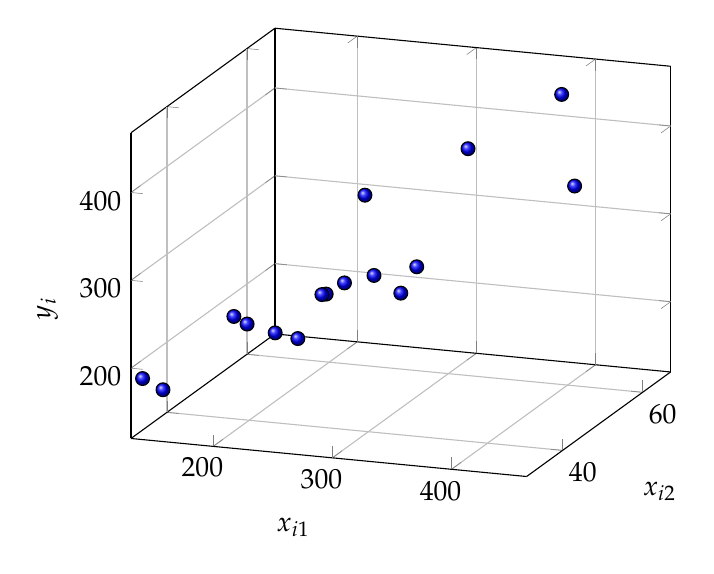
\begin{tikzpicture}
			\begin{axis}[
				view={20}{20}, % Set the view angle
				xlabel=$x_{i1}$,
				ylabel=$x_{i2}$,
				zlabel=$y_i$,
				grid=major,
			]
			% Scatter plot data points
			\addplot3[
				only marks,
				mark=ball,
				mark size=2.5,
			]
			coordinates {
				(278, 36, 287)
				(252, 31, 256)
				(344, 35, 300)
				(134, 33, 182)
				(215, 35, 248)
				(261, 40, 271)
				(131, 39, 149)
				(463, 43, 411)
				(167, 46, 214)
				(298, 42, 291)
				(230, 60, 314)
				(293, 67, 352)
				(290, 37, 298)
				(271, 31, 252)
				(385, 63, 439)
				(354, 36, 328)
			};
			% % Define the equation of the plane: ax + by + cz + d = 0
			% \addplot3[
			% 	surf,
			% 	opacity=0.5,
			% 	faceted color=blue,
			% 	shader=interp,
			% 	domain=200:400,
			% 	domain y=20:60,
			% ] {0.7*x + 2.6*y - 11.3};
			\end{axis}
		\end{tikzpicture}
	\end{minipage}	
	\caption{Data points in $\R^3$.}
	\label{fig:3d-data-points}
\end{figure}

We can put some meaning to these data. For example, suppose a company is selling
a product, and we have 16 populations of people labeled $0$ through $15$. The
values $x_{i1}$ are the population sizes in $100$s of people; the values
$x_{i2}$ are the average yearly income in €$1000$ per capita; and the values
$y_i$ are the number of sales of the product. (There might be dependencies
between population size and average income, but our model treats them as
independent.)

It looks like though there is a plane of best fit for the data---thanks to the
suggestive viewing angle. Our goal is to find a plane, given by 
\begin{align*} 
	y = b_0 + b_1x_1 + b_2x_2. 
\end{align*} 
We can just do what we did last time. That is, for 
\begin{align*}
	X &= \begin{pmatrix}
		1 & x_{11} & x_{12} \\ 
		1 & x_{21} & x_{22} \\
		\vdots & \vdots & \vdots \\
		1 & x_{n1} & x_{n2} 
	\end{pmatrix}, & 
	Y &= \begin{pmatrix}
		y_1 \\ y_2 \\ \vdots \\ y_n
	\end{pmatrix}, & 
	B &= \begin{pmatrix}
		b_0 \\ b_1 \\ b_2
	\end{pmatrix},
\end{align*}
we need to solve for $B$ in the equation
\begin{align*}
	X^{\tr} X B &= X^{\tr} Y .	
\end{align*}
Thus, if $X^{\tr}X$ is invertible, there is a unique $B$, which is equal to
$(X^{\tr}X)^{-1}X^{\tr}Y$. For our example, we have 
\begin{align*}
	X^{\tr}X &= \begin{pmatrix}
		16 &    4366 &     674 \\
		4366 & 1309480 &  187024 \\
		674 &  187024 &   30330
	\end{pmatrix}, & 
	X^{\tr}Y &= \begin{pmatrix}
		4592 \\
		1343400 \\
		200571
	\end{pmatrix}.
\end{align*}
Therefore, the plane of best fit is approximately
\begin{align*}
	y &= -11.3 + 0.7x_1 + 2.6x_2.
\end{align*}
Putting all the data together we have a plane of best fit as seen in
\Cref{fig:plane-and-scatter}.

\begin{figure}[h]
	\centering
	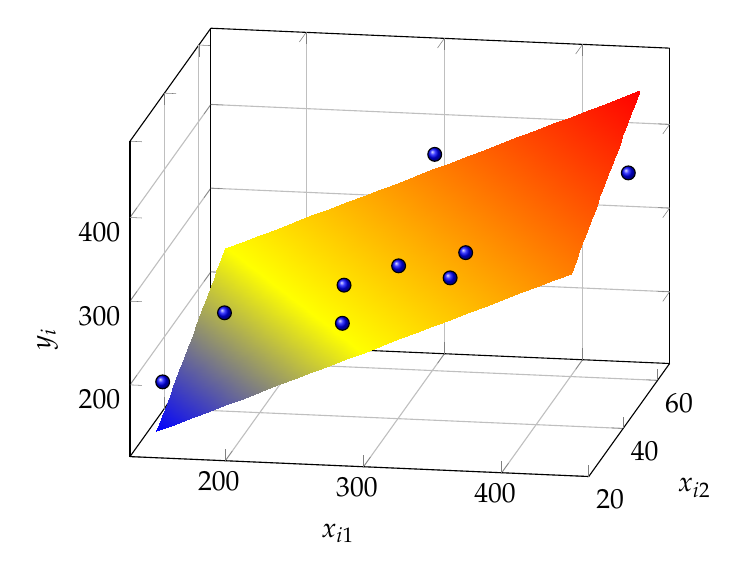
\begin{tikzpicture}
		\begin{axis}[
			view={10}{20}, % Set the view angle
			xlabel=$x_{i1}$,
			ylabel=$x_{i2}$,
			zlabel=$y_i$,
			grid=major,
		]
		% Scatter plot data points
		\addplot3[
			only marks,
			mark=ball,
			mark size=2.5,
		]
		coordinates {
			% (278, 36, 287)
			% (252, 31, 256)
			(344, 35, 300)
			% (134, 33, 182)
			% (215, 35, 248)
			(261, 40, 271)
			(131, 39, 149)
			(463, 43, 411)
			(167, 46, 214)
			(298, 42, 291)
			% (230, 60, 314)
			(293, 67, 352)
			% (290, 37, 298)
			(271, 31, 252)
			% (385, 63, 439)
			(354, 36, 328)
		};
		% Define the equation of the plane: ax + by + cz + d = 0
		\addplot3[
			surf,
			opacity=1,
			shader=interp,
			domain=150:450,
			domain y=20:60,
		] {0.7*x + 2.6*y - 11.3};
		\end{axis}
	\end{tikzpicture}
	\caption{Data points together with the plane of best fit.}
	\label{fig:plane-and-scatter}
\end{figure}

\subsection{Hyperplane of best fit}

Now we go to the general case. Suppose we have $p-1$ independent variables and
$1$ dependent variable, where $p\geq 2$. We assume we have $n$ data points of the form 
\[ 
	\left( x_{i1}, x_{i2}, \dots, x_{i,p-1}, y_1 \right) \in \R^p. 
\] 
The least squares fitting for these data is a hyperplane of the form 
\[ 
	y = b_0 + b_1 x_1 + b_2x_2 + \cdots + b_{p-1}x_{p-1}. 
\] 

To solve for the values $b_i$, we do as we did before. We define matrices 
\begin{align*}
	X &= \begin{pmatrix}
		1 & x_{11} & x_{12} & \cdots & x_{1,p-1} \\
		1 & x_{21} & x_{22} & \cdots & x_{2,p-1} \\
		\vdots & \vdots & \vdots & \ddots & \vdots \\
		1 & x_{n1} & x_{n2} & \cdots & x_{n,p-1} 
	\end{pmatrix}, & 
	Y &= \begin{pmatrix}
		y_1 \\ y_2 \\ \vdots \\ y_n 
	\end{pmatrix}, & 
	B &= \begin{pmatrix}
		b_0 \\ b_1 \\ \vdots \\ b_{p-1}
	\end{pmatrix}. 
\end{align*}
As before, the values we want are given by the equation 
\begin{align}\label{eqn:general-OLS}
	X^{\tr} X B &= X^{\tr} Y.
\end{align}

\subsection{Why \Cref{eqn:general-OLS} works}

The heart of least squares is (Euclidean) distance. The distance between two points $x = (x_1,\dots, x_p)$ and $y=(y_1,\dots, y_p)$ in $\R^p$ is 
\begin{align*}
	d(x, y) = \| x - y \| = \sqrt{(x_1 - y_1)^2 + (x_2 - y_2)^2 + \cdots + (x_p - y_p)^2}. 
\end{align*}
For a vector $v=(v_1,\dots, v_p)\in\R^p$, the \textbf{length} of $v$ is 
\begin{align*}
	\| v \| = d(0, v) = \sqrt{v_1^2 + v_2^2 + \cdots + v_p^2}.
\end{align*}
Recall that the dot product of two (column) vectors $u$ and $v$ is 
\[ 
	u\cdot v = u^{\tr} v = u_1v_1 + u_2v_2 + \cdots + u_pv_p.
\] 
Thus, the length of $v$ is $\| v \| = \sqrt{v\cdot v}$; in other words $\| v\|^2
= v\cdot v$. In addition, if $u\cdot v = 0$, we say that $u$ and $v$ are
\textbf{orthogonal} (or perpendicular).

The goal of least squares is to \textit{minimize distance}; more specifically to
minimize $\|Y - XB\|$. Note that the column vector $Y$ has entries that are the
\textit{actual $y_i$ values}, and the column vector 
\begin{align*}
	XB &= \begin{pmatrix}
		B\cdot (1, x_{11}, x_{12}, \dots, x_{1,p-1}) \\ 
		B\cdot (1, x_{21}, x_{22}, \dots, x_{2,p-1}) \\ 
		\vdots \\
		B\cdot (1, x_{n1}, x_{n2}, \dots, x_{n,p-1}) 
	\end{pmatrix} = \begin{pmatrix}
		b_0 + b_1x_{11} + b_2x_{12} + \cdots + b_{p-1}x_{1,p-1} \\ 
		b_0 + b_1x_{21} + b_2x_{22} + \cdots + b_{p-1}x_{2,p-1} \\ 
		\vdots \\
		b_0 + b_1x_{n1} + b_2x_{n2} + \cdots + b_{p-1}x_{n,p-1}
	\end{pmatrix}
\end{align*}
Therefore, $\| Y - XB \|$ is the square root of a sum of squares of the form 
\begin{align*}
	y_i - b_0 + b_1x_{i1} + b_2x_{i2} + \cdots + b_{p-1}x_{i,p-1}.
\end{align*}
Hence minimizing $\| Y - XB \|$ is the same as minimizing $\| Y - XB \|^2$,
which is a sum of \textit{squares}.

\begin{prop}
	The minimal distance $\| Y - XB \|$ is achieved by solving for $B$ in 
	\[ 
		X^{\tr} X B = X^{\tr} Y.
	\] 
\end{prop}

\WEEK{2}

\begin{proof} 
	Consider the subspace $U = \{Xu ~|~ u\in\R^p\}$ of $\R^n$, and observe that
	our desired solution $XB$ is contained in $U$. Since $\| Y - XB \|$ is
	minimal, we must have that the vector $Y - XB$ is orthogonal to all vectors
	contained in $U$.\footnote{To see why this is true, see Section 6.3.1 of
	\cite{ILA}, which is all about orthogonal decompositions.} That is, $(Xu)
	\cdot (Y - XB) = 0$ for all $u\in\R^p$. In other words, we have for all
	$u\in \R^p$,
	\begin{align*} 
		0 = (Xu)^{\tr} (Y - XB) &= u^{\tr} X^{\tr}(Y - XB) \\
		&= u^{\tr} \left(X^{\tr}Y - X^{\tr}XB\right).
	\end{align*}
	Because $u^{\tr} \left(X^{\tr}Y - X^{\tr}XB\right)=0$ for all $u\in \R^p$,
	it follows that $X^{\tr}Y - X^{\tr}XB=0$. 
\end{proof}

\subsection{In class exercises pt. II}

\begin{enumerate}
	\item Determine $X^{\tr}X$ and $X^{\tr}Y$ with
	\begin{align*}
		X &= \begin{pmatrix}
			1 & x_{11} & x_{12} & \cdots & x_{1,p-1} \\
			1 & x_{21} & x_{22} & \cdots & x_{2,p-1} \\
			\vdots & \vdots & \vdots & \ddots & \vdots \\
			1 & x_{n1} & x_{n2} & \cdots & x_{n,p-1} 
		\end{pmatrix}, & 
		Y &= \begin{pmatrix}
			y_1 \\ y_2 \\ \vdots \\ y_n 
		\end{pmatrix}.
	\end{align*}
	\item Using (1) and by taking partial derivatives of 
	\begin{align}\label{eqn:S-function}
		S(b_0, \dots, b_{p-1}) &= \sum_{i=1}^n (y_i - (b_0 + b_1x_{i1} + b_2x_{i2} + \cdots + b_{p-1}x_{i,p-1}))^2,
	\end{align}
	show that the hyperplane of best fit is obtained by solving
	$X^{\tr}XB=X^{\tr}Y$. (You could try this for $p=3$ first.)
\end{enumerate}

\subsection{Nonlinear fittings}\label{sec:nonlinear-fittings}

Although all of our examples so far have been linear fittings, we will
demonstrate that least squares fittings works in the nonlinear case. What is
important is that we have a candidate equation to fit. In the linear cases, we
tried to fit 
\[ 
	y = b_0 + b_1x_1 + b_2x_2 + \cdots + b_{p-1}x_{p-1}.
\] 

Suppose we have the following data as given in \Cref{fig:nonlinear-data}.
Instead of trying to fit the line $y=b_0+b_1x$, we could try to fit the
parabola: 
\[ 
	y = b_0 + b_1x + b_2x^2. 
\] 
We can treat this the same way as before. Of course the quantities $x$ and $x^2$ are \textit{not} independent, but we can ignore this. Set 
\begin{align*} 
	x_{i1} &= x_i, & x_{i2} &= x_i^2.
\end{align*} 
Therefore, the hyperplane of best fit for the data $(x_{i1}, x_{i2}, y_i)$ will
give us the parabola of best fit. \textit{Try this on your own!} 

\begin{figure}[h]
	\centering
	\begin{minipage}{0.3\textwidth}
		\centering
		\begin{tabular}{cc}
			$x_i$ & $y_i$ \\ \hline
			2.27 & 2.50 \\
			5.06 & -16.13 \\ 
			1.45 & 4.23 \\ 
			5.89 & -22.46 \\
			0.48 & 1.37 \\ 
			-0.22 & 0.86 \\ 
			1.44 & 11.85 \\ 
			-1.77 & -14.71 \\ 
			2.45 & 9.42 \\ 
			-1.54 & -14.07 \\ 
			7.55 & -55.62 \\ 
			1.76 & 4.45 \\ 
			5.16 & -19.56 \\ 
			3.26 & -2.79 \\
			3.23 & 5.20 \\
			0.85 & 8.09
		\end{tabular}
	\end{minipage}~%
	\begin{minipage}{0.65\textwidth}
		\centering
		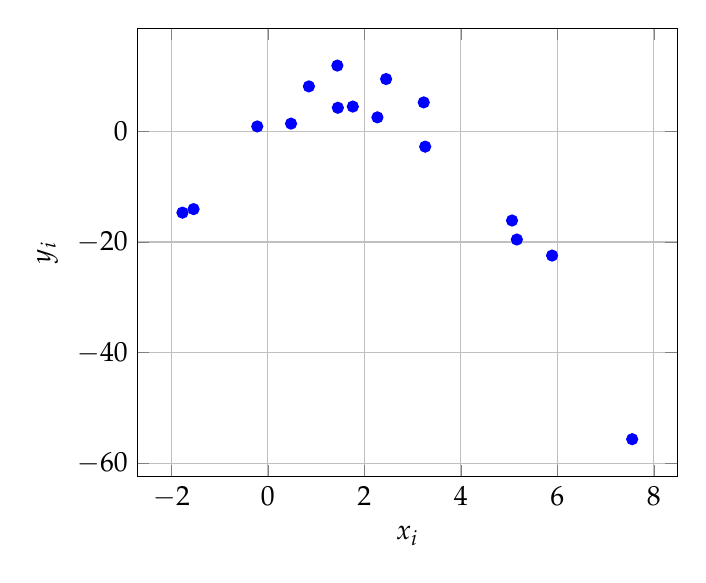
\begin{tikzpicture}
			\begin{axis}[
				xlabel=$x_i$,
				ylabel=$y_i$,
				grid=both,
			]
			\addplot[only marks, mark=*, mark size=2pt, color=blue] coordinates {
				(2.27, 2.50)
				(5.06, -16.13)
				(1.45, 4.23)
				(5.89, -22.46)
				(0.48, 1.37)
				(-0.22, 0.86)
				(1.44, 11.85)
				(-1.77, -14.71)
				(2.45, 9.42)
				(-1.54, -14.07)
				(7.55, -55.62)
				(1.76, 4.45)
				(5.16, -19.56)
				(3.26, -2.79)
				(3.23, 5.20)
				(0.85, 8.09)
			};
			\end{axis}
		\end{tikzpicture}
	\end{minipage}
	\caption{Data points demonstrating a nonlinear relationship.}
	\label{fig:nonlinear-data}
\end{figure}

So one can fit any hypersurface $y=f(x_1,\dots, x_{p-1})$ to the given data. The
function $f$ in this case is called the \textbf{regression function}. This
general method of analysis is known as \textbf{regression analysis}. A few
questions arise:
\begin{itemize}
	\item Which surface is ``best''?
	\item How can we quantify ``best''?
	\item Even in the line case $(p=2)$, how can we quantify how well data fits
	our line? 
\end{itemize}

\WEEK{3}

\subsection{Coefficient of determination ($R^2$ values)}

We are going to make precise how well our hyperplane fits our data. Recall that
hyperplanes can be replaced by hypersurfaces; see \Cref{sec:nonlinear-fittings}.
First we establish some notation. Suppose we have $n$ data points $(x_{i1},
x_{i2}, \dots, x_{i,p-1}, y_i)\in \R^p$. Then we define  
\begin{align*}
	\text{(Fitted value)} & & \widehat{y}_i &= b_0 + b_1x_{i1} + b_2 x_{i2} + \cdots + b_{p-1} x_{i,p-1}, \\
	\text{(Residual)} & & e_i &= y_i - \widehat{y}_i, \\
	\text{(Sample mean)} & & \overline{y} &= \frac{1}{n}\sum_{i=1}^n y_i.
\end{align*}
These yield vectors in $\R^n$ as follows 
\begin{align*}
	\widehat{Y} &= \begin{pmatrix}
		\widehat{y}_1 \\ \vdots \\ \widehat{y}_n
	\end{pmatrix} = XB, & 
	E &= \begin{pmatrix}
		e_1 \\ \vdots \\ e_n
	\end{pmatrix} = Y - \widehat{Y}, & 
	\overline{Y} &= \begin{pmatrix}
		\overline{y} \\ \vdots \\ \overline{y}
	\end{pmatrix} = \overline{y} \begin{pmatrix}
		1 \\ \vdots \\ 1 
	\end{pmatrix}. 
\end{align*}

From our $n$ data points, we have three points in $\R^n$ given by $Y$,
$\widehat{Y}$, and $\overline{Y}$. Three points always lie on a plane, so the
three point determine a triangle on such a plane. What does this triangle look
like? If it is a triangle (and not a line or a single point), then the next
lemma proves it must be a right triangle.

\begin{lem}\label{lem:orthog}
	The vectors $E = Y - \widehat{Y}$ and $\widehat{Y}-\overline{Y}$ are
	orthogonal.
\end{lem}

\begin{proof}
	Suppose $X^{\tr}XB = X^{\tr}Y$. We need to prove two equations. For the
	first, 
	\begin{align*}
		0 &= X^{\tr}(Y - XB) = X^{\tr}(Y - \widehat{Y}) = X^{\tr}E.
	\end{align*}
	Hence, $X^{\tr}E=0$. For the second, 
	\begin{align*}
		\overline{Y}^{\tr}E &= \overline{y} \sum_{i=1}^n (y_i - \widehat{y}_i) \\
		&= \overline{y} \sum_{i=1}^n (y_i - (b_0+b_1x_{i1} + b_2x_{i2} + \cdots + b_{p-1}x_{i,p-1})) \\
		&= -\dfrac{\overline{y}}{2} \cdot \dfrac{\partial S}{\partial b_0} = 0,
	\end{align*}
	where $S$ is defined in \Cref{eqn:S-function}, so $\overline{Y}^{\tr}E=0$.
	Thus, we have 
	\begin{align*}
		(\widehat{Y} - \overline{Y}) \cdot E &= (XB)^{\tr} E - \overline{Y}^{\tr}E = 0. \qedhere
	\end{align*}
\end{proof}

\begin{remark}
	One can simplify the proof for \Cref{lem:orthog} by applying an isometry to
	the data, so that $\overline{y} = 0$. That is, one only needs to prove that
	$E$ and $\widehat{Y}$ are orthogonal.
\end{remark}

The lengths of the differences of the vectors are important and have names: 
\begin{align*} 
	\text{(Sums of Squares Total -- SST)} &: \|Y - \overline{Y} \|^2, \\
	\text{(Sums of Squares Error -- SSE)} &: \| Y - \widehat{Y}\|^2, \\
	\text{(Sums of Squares Regression -- SSR)} &: \| \widehat{Y} - \overline{Y}\|^2 .
\end{align*} 
The value $SST$ measures the \textit{total variability} of the data set. For
example, $\sqrt{SST} = \| Y - \overline{Y} \|$ is the distance from the actual
data $Y$ to the sample mean $Y$. Using the same ideas, we can see that $SSE$
measures the error of our regression and that $SSR$ measures the distance from
our regression to the sample mean. 

\begin{prop}\label{prop:SS-values}
	\[ 
		SST = SSE + SSR. 
	\] 
\end{prop}

\begin{proof}
	Apply \Cref{lem:orthog} and the Pythagorean Theorem:
	\begin{align*} 
		\| Y - \overline{Y} \|^2 &= \| Y - \widehat{Y}\|^2 + \| \widehat{Y} - \overline{Y} \|^2.  \qedhere
	\end{align*} 
\end{proof}

Now we can describe a quantity that measures how good our regression fits the
given data. 

\begin{defn}
	The \textbf{coefficient of determination} (also known as the
	\textbf{$R^2$-value}) is 
	\begin{align*} 
		R^2 &= \dfrac{SSR}{SST} = \dfrac{\|\widehat{Y} - \overline{Y}\|^2}{\| Y - \overline{Y}\|^2} .
	\end{align*} 
\end{defn}

\begin{prop}
	$0\leq R^2 \leq 1$.
\end{prop}

\begin{proof}
	Since each SST and SSR are squares, they are nonnegative. By
	\Cref{prop:SS-values}, we have $0\leq SSR\leq SST$.
\end{proof}

\subsubsection{What do the extremes means?}

The one case where $R^2$ is meaningless is when $SST=0$. This implies both
$SSR=SSE=0$. Moreover, $Y = \overline{Y} = \overline{y} \mathbbm{1}$, where
$\mathbbm{1}$ is the all ones column vector. Hence, every data point $y_i$ is
the same and, therefore, equal to the mean. Let's never return to this case.

We can have $SSR=0$, which is equivalent to $R^2=0$. This implies that $\|
\widehat{Y} - \overline{Y}\|^2= 0$, so that $\widehat{Y} = \overline{Y}$. In
other words, our prediction $\widehat{y}_i$ is just simply the mean. This means
we have not found any relationship between the independent variables and the
dependent variables. 

In the other extreme we have $SSR=SST$, which is equivalent to $R^2=1$. This
implies that $Y = \widehat{Y}$, so the given data lies (exactly) on the surface
given by $y=f(x_1,\dots, x_{p-1})$. That is, the regression function exactly
predicts the data. 

To summarize, when $R^2=0$, we cannot deduce any relationship between the
independent and dependent variables, and when $R^2=1$, we understand completely
the relationship between the independent and dependent variables. Very roughly
speaking, the $R^2$ can be thought of as the ratio of how well the regression
fits the data. 

\subsection{In class exercises pt. III}

\begin{enumerate}
	\item Prove the following.
	\begin{enumerate}
		\item $\| \overline{Y} \|^2 = n\overline{y}$.
		\item $Y \cdot \overline{Y} = \widehat{Y}\cdot \overline{Y} = \| \overline{Y} \|^2$.
		\item $Y\cdot \widehat{Y} = \| \widehat{Y} \|^2$.
	\end{enumerate}
	\item Use (1) to show that 
	\begin{enumerate}
		\item $SST = \|Y\|^2 - \|\overline{Y}\|^2$,
		\item $SSE = \|Y\|^2 - \| \widehat{Y} \|^2$,
		\item $SSR = \| \widehat{Y} \|^2 - \| \overline{Y} \|^2$.
	\end{enumerate}
	\item What are the $R^2$ values for the examples above?
\end{enumerate}


\section{Principal component analysis}

Principal component analysis (PCA) is a power method of analysis that comes
standard in all data science tool kits. With little effort, one can reduce a
complex data set to data that we can more easily see structure. More
specifically, the goal of PCA is to find the ``best'' basis to express the data.
In other words, our initial reference frame may not be the one that best
expresses the structure of our data---PCA is a method to find the ``best''
reference frame.

\subsection{Introducing PCA}

We will start with a toy example, where the analysis is quite simple. Suppose we
have many many data points in $\R^2$ as seen in \Cref{fig:pca-example}.

\begin{figure}[h]
    \centering
    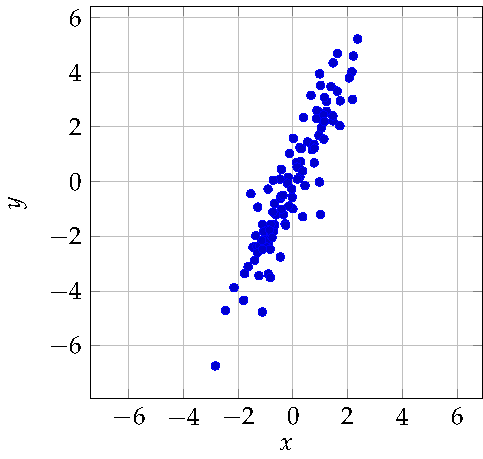
\includegraphics{graphics/pca_example.pdf}
    \caption{Some data in $\mathbb{R}^2$.}
	\label{fig:pca-example}
\end{figure}

Let's assume that our data points live in $\R^m$, so that $m=2$ in
\Cref{fig:pca-example}. Suppose we write those data points in an $m\times n$
matrix $X$. Our current (and default) basis is $\{(1,0, \dots, 0), (0,1, 0,
\dots, 0), \dots, (0,\dots, 0,1)\}$, and we want a basis $\{p_1,p_2, \dots,
p_m\}$ that better reflects the structure of our data. That is, we want an
$m\times m$ matrix $P$, whose rows are the $p_i$, that provides us a better
reference frame. Therefore, we want to transform our data $X$ into a new data
set $Y$ such that 
\[ 
	PX = Y. 
\] 
The columns of $X$ are the ``old'' data, and the columns of $Y$ are the ``new''
data. If the $p_i$ are row vectors and the $x_i$ column vectors, then we want 
\[ 
	PX = \begin{pmatrix} 
		p_1 \\ p_2 \\ \vdots \\ p_m 
	\end{pmatrix} \begin{pmatrix} 
		x_1 & x_2 & \cdots x_n
	\end{pmatrix} = \begin{pmatrix}
		p_1\cdot x_1 & p_1\cdot x_2 & \cdots & p_1\cdot x_n \\
		p_2 \cdot x_1 & p_2 \cdot x_2 & \cdots & p_2 \cdot x_n \\ 
		\vdots & \vdots & \ddots & \vdots \\
		p_m \cdot x_1 & p_m \cdot x_2 & \cdots & p_m \cdot x_n 
	\end{pmatrix}. 
\] 
Thus, if the columns of $Y$ are written $y_i$, we have 
\begin{align}\label{eqn:proj-P}
	y_i &= \begin{pmatrix}
		p_1 \cdot x_i \\ p_2 \cdot x_i \\ \vdots \\ p_m \cdot x_i
	\end{pmatrix}. 
\end{align}

Back to our example from \Cref{fig:pca-example}. We want data with a high
\textit{signal-to-noise} (SNR) ratio as to minimize noise. Assuming our data in
\Cref{fig:pca-example} was collected reasonably well, the direction of largest
variance is the direction of most interesting dynamics. Therefore, the variance
of signal, $\sigma_{\mathrm{s}}^2$, would correspond to the length of the
orange vector in \cref{fig:pca-example2} pointing to the top right, and the
variance of the noise, $\sigma_{\mathrm{n}}^2$, would correspond to the length
of the orange vector pointing to the top left. 

\begin{figure}[h]
    \centering
    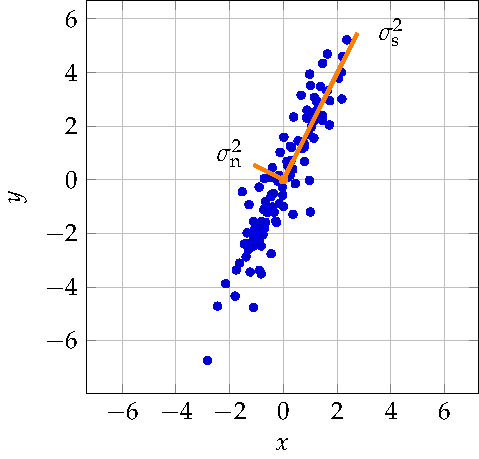
\includegraphics{graphics/pca_example2.pdf}
    \caption{Signal and noise variances represented graphically.}
	\label{fig:pca-example2}
\end{figure}

Note also that in \Cref{fig:pca-example2} knowing the $x$ value gives one a good
approximation for the $y$ value and vice versa. In this case, we might say that
the data has a moderate amount of redundancy, whereas if the data points had a
much higher $R^2$ value to its line of best fit, we would say the data have high
redundancy. (And if the data had a much lower $R^2$ value, we would say the data
have low redundancy.) One of the aims of PCA is to lower redundancy. For the
$2$-dimensional case, this is simple---take the line of best fit, but for
arbitrarily higher dimensions, this is not obvious. 

\WEEK{4}


Suppose we have $n$ measurements of the same kind (like length)
\[ 
	U = \{u_1, u_2, \dots, u_n\} \qquad \text{ and } \qquad V = \{v_1, v_2, \dots, v_n\}
\] 
\textbf{with mean equal to} $\mathbf{0}$. The \textit{variances} are equal to 
\begin{align*} 
	\sigma_U^2 &= \dfrac{1}{n} \sum_{i=1}^n u_i^2, & \sigma_V^2 &= \dfrac{1}{n} \sum_{i=1}^n v_i^2 .
\end{align*} 
The \textit{covariance} between the data sets $U$ and $V$ is 
\begin{align*}
	\sigma_{UV}^2 &= \dfrac{1}{n} \sum_{i=1}^n u_iv_i.
\end{align*}
The covariance measures the degree of the linear relationship between the two
variables. Thus, a large positive value would imply that the data are positively
correlated, and a large negative value would imply negatively correlated. And
$\sigma_{UV}^2= 0$ if and only if the data $U$ and $V$ are uncorrelated.
Moreover the absolute magnitude of the covariance measures the degree of
redundancy. 

If instead we wrote $u = (u_1, u_2, \dots, u_n)$ and $v= (v_1,v_2, \dots, v_n)$
as row vectors, then 
\begin{align}\label{eqn:vec-covar}
	\sigma_{uv}^2 = \dfrac{1}{n} u v^{\tr}. 
\end{align} 
We generalize from two vectors to $m$ vectors. Write 
\begin{align*}
	X = \begin{pmatrix}
		x_1' \\ x_2' \\ \vdots \\ x_m'
	\end{pmatrix}
\end{align*}
where $x_i'$ is a row vector. Note that the rows of $X$ correspond to
measurements of a particular type, and the columns of $X$ correspond to all
measurements of a particular trial. In other words, our data points are the
columns of $X$, and each entry of a data point is a measurement of a particular
type. 

Using \Cref{eqn:vec-covar}, we define the
\textbf{covariance matrix} of $X$ to be 
\begin{align*} 
	C_X &= \dfrac{1}{n} XX^{\tr} .
\end{align*} 

\begin{lem}\label{lem:covariance-properties}
	\hfill 
	\begin{enumerate}
		\item The matrix $C_X$ is symmetric. That is, $C_X = C_X^{\tr}$.
		\item The diagonal entries of $C_X$ are variances.
		\item The off-diagonal entries of $C_X$ are covariances.
	\end{enumerate}
\end{lem}

Recall our goal is to find a new (and better) basis $\{p_1, p_2, \dots, p_m\}$.
Namely, we want an invertible matrix $P$ to turn our data $X$ into a data set
$Y$ where we can better understand the structure. If we could do this on the
level of covariance matrices, then we could pick an ideal covariance matrix, one
where the diagonal entries are large in absolute magnitude and where the
off-diagonal entries are small in absolute magnitude. (Variances being high in
magnitude suggest interesting dynamics, and covariances low in magnitude suggest
low redundancy.) In other words, we would like to find a matrix $P$ such that 
\begin{align}\label{eqn:cov-Y}
	C_Y &= \begin{pmatrix}
		\lambda_1 & 0 & \cdots & 0 \\
		0 & \lambda_2 & \cdots & 0 \\
		\vdots & \vdots & \ddots & \vdots \\
		0 & 0 & \cdots & \lambda_m
	\end{pmatrix},
\end{align}
where $Y = PX$. Typically we have $\lambda_1 \geq \lambda_2 \geq \cdots \geq \lambda_m$.

The main work of PCA is finding such a matrix $P$. We will describe how to
construct such a $P$ later, but let us return to our running example.  

The first principal component is in the direction of the largest variance, and
the second principal component is in the orthogonal direction. So in $\R^2$,
this is quite simple. Although we have not given all the data point explicitly,
the covariance matrix is 
\begin{align*}
	C_X &= \begin{pmatrix}
		1.27 & 2.52 \\
		2.52 & 5.95
	\end{pmatrix}.
\end{align*}
The slope of the line in the direction of the highest variance is 1.98, and it
passes through the point $(0,0)$. By rotating and permuting, we get 
\begin{align*}
	P &= \begin{pmatrix}
		0.40 & 0.92 \\ 0.92 & -0.40 
	\end{pmatrix},
\end{align*}
and the graph of the data $Y = PX$ is seen in \Cref{fig:pca-example3}.

\begin{figure}[h]
    \centering
    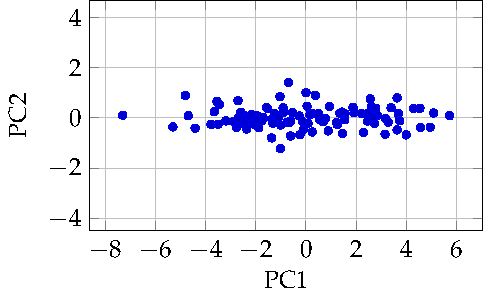
\includegraphics{graphics/pca_example_rotated.pdf}
    \caption{A new basis for our data.}
	\label{fig:pca-example3}
\end{figure}

\begin{remark}
	There is a whole art of scaling data in a pre-processing stage that we will
	not explore in this course. Basically, if one variable ranges between $\pm
	10$ and another $\pm 10^3$, the second variable will bias the process simply
	by its scale. There are many different methods to rescale the data as not to
	lose (too much) information. \textit{Throughout we will assume our data has
	roughly the same scale and not worry about rescaling}, but in practice this
	is an important issue.
\end{remark}

\subsubsection{Assumptions of PCA}

Before we close this introduction to PCA, let us come back to some of the
assumptions we have made along the way. There are three key assumptions we have
made in introducing PCA. We will not focus much on these, but users of PCA
should know that assumptions have been made. These statements may not
necessarily hold for a particular data set. 

\begin{enumerate}
	\item \textit{Linearity.} 
	
	This allows us to reframe the problem as a change of basis problem. 

	\item \textit{Large variance is important (and $SNR>1$).}
	
	This can be a very strong assumption and really needs to take into account
	how the data was collected. 
	
	\item \textit{Principal components are orthogonal.}
	
	This is not always the case, but orthogonality allows us to use linear
	algebra. 
\end{enumerate}

\subsection{In class exercises pt. IV}

\begin{enumerate}
	\item 
	\begin{enumerate}
		\item Show that $C_X$ is symmetric. 
		\item Prove that the diagonal entries of $C_X$ are variances and the
		off-diagonal entries are covariances. 
	\end{enumerate}
	\item Suppose $X$ is an $m\times n$ matrix with sample mean
	$\overline{x}\in\R^m$. Let $X'$ be the shifted data of $X$, so that its
	sample mean is $0$. What is $C_{X'}$ in terms of $X$ and $\overline{x}$?
\end{enumerate}

\subsection{Performing PCA}\label{sec:perform-pca}

At the heart of performing PCA in practice is the following question. Recall
that $C_Y$ is a diagonal matrix; see the discussion around \Cref{eqn:cov-Y}.

\begin{quest} 
	What is the relationship between $C_X$ and $C_Y$ if $Y = PX$? 
\end{quest}

\begin{proof}
	From above, we have
	\begin{align*}
		C_Y &= \dfrac{1}{n} YY^{\tr} = \dfrac{1}{n} (PX)(PX)^{\tr} = P C_X P^{\tr}. \qedhere
	\end{align*}
\end{proof}

In order to perform a PCA, we need to find a matrix $P$ such that $PC_XP^{\tr}$
is diagonal. Importantly, we do not want to change the variances, so we want $P$
to be \textit{distance preserving}; that is, we want $P$ to satisfy
\begin{align}\label{eqn:dist-preserve}
	\| Pv \| &= \| v\|
\end{align}
for all vectors $v\in\R^m$. We say such a matrix $P$ is an \textbf{isometry}. We
can take \Cref{eqn:dist-preserve} and massage it, so that $P$ must satisfy 
\begin{align*}
	v^{\tr} P^{\tr} P v &= (Pv)\cdot (Pv) = v\cdot v = v^{\tr} v
\end{align*}
for all $v\in \R^m$. Since this needs to hold for all vectors, it must hold for
all pairs of basis vectors $(e_i,e_j)$ for all $i,j\in\{1,\dots, m\}$. Thus,
distance preserving is equivalent to $P^{\tr}P = I_m$, but these matrices are
called \textbf{orthogonal}. (Note: pairs of distinct columns of such a matrix
$P$ are pairwise orthogonal. Can you prove this?!) 

\WEEK{5}

Let us bring this back to the equation we established. We want $P$ to be an
orthogonal matrix such that 
\begin{align}\label{eqn:CY-CX}
	C_Y = PC_XP^{\tr} .
\end{align} 
Moreover, we want $C_Y$ to be a diagonal matrix. Since $P^{\tr}P=I_m$, it
follows that $P^{-1} = P^{\tr}$, so using this identity we have 
\begin{align*}
	C_Y &= PC_XP^{-1}.
\end{align*}
Since $C_Y$ is diagonal, this is accomplished through
\textit{eigendecomposition}. Therefore, the rows of $P$ are eigenvectors, and
the diagonal entries of $C_Y$ are eigenvalues.

All the entries of $C_Y$ are \textit{real}, and we know that some matrices have
complex eigenvalues. For example, the matrix 
\begin{align*}
	\begin{pmatrix}
		0 & -1 \\ 1 & 0 
	\end{pmatrix}
\end{align*}
has eigenvalues $i$ and $-i$, for $i=\sqrt{-1}$. 
\begin{quest}\label{quest:PCA-possible}
	Is it always possible to find a real matrix $P$ such that \Cref{eqn:CY-CX}
	holds?
\end{quest}
The answer to \Cref{quest:PCA-possible} is ``Yes,'' and we will prove it later.
For now, let us assume it is always possible. 

\medskip

We give a recipe for cooking up the principal components.
\begin{description}
	\item[Given:] $n$ data points $x_i\in\R^m$ (of roughly the same scale),
	\item[Return:] $m$ principal components.
\end{description}
\begin{enumerate}
	\item Compute the mean of each coordinate: $\mu_j = \sum_i x_{ij}$,
	\item Organize the normalised data into a matrix $X = (x_{ij} - \mu_j)$,
	\item Compute the covariance matrix $C_X$ of $X$,
	\item Compute the eigenvectors of $C_X$, and sort them based on their
	eigenvalues: largest is first and smallest is last.
	\item Return the (ordered) orthonormal basis of eigenvectors. 
\end{enumerate}

PCA is a phrase used for this algorithm together with its analysis, and one of
the main ways PCA is performed is by taking only the first $k$ principal
components (rather than all $m$). Here, $k$ is usually determined by the
\textit{eigenvalues}. 

Both $C_X$ and $C_Y$ have the same eigenvalues: $\lambda_1 \geq \lambda_2 \geq
\cdots \geq \lambda_m$. Since the trace of matrix is the sum of its eigenvalues,
both $C_X$ and $C_Y$ have the same trace. In other words, 
\begin{align*}
	\mathrm{tr}(C_X) &= \sum_{i=1}^m \lambda_i,
\end{align*}
and by \Cref{lem:covariance-properties}, the sum of the variances is the sum of
the eigenvalues. Because we view variability as an important measurement to keep
track of, we can choose a $k$ that both maximizes the amount of variability
``seen'' and while minimizing the value of $k$. This is a bit more of an art
than a science, but one general rule could be to choose the smallest $k$ such
that 
\begin{align} \label{eqn:k-rule}
	\dfrac{\sum_{i=1}^k\lambda_i}{\sum_{i=1}^m\lambda_i} \geq 0.95.
\end{align} 
For such a $k$, one might say that the first $k$ principal components capture
$95\%$ of the total variability.

\begin{quest}\label{quest:small-PC}
	Are the principal components $k+1$ through $m$ useless? 
\end{quest}

\subsection{Projections}

The answer to \Cref{quest:small-PC} is essentially ``Yes'', and it can be
helpful to consider an idealised example. 

Recall that $X$ is our $m\times n$ matrix whose columns are our $n$ data points
in $\R^m$. The matrix $P$ is obtained from the eigenvectors of $C_X$, which are
the rows of $P$, and $Y=PX$. Moreover, $P$ is an orthogonal matrix. Suppose $k <
m$ and 
\[ 
	\lambda_{k+1} = \lambda_{k+2} = \cdots = \lambda_m = 0. 
\]
Therefore, we have 
\[ 
	C_Y = \begin{pmatrix} 
		\lambda_1 & & & & & \\
		& \ddots & & & \\
		& & \lambda_k & & & \\
		& & & 0 & & \\
		& & & & \ddots & \\
		& & & & & 0
	\end{pmatrix} .
\] 

\begin{remark}\label{rem:tail-zeroes}
	In this situation, $y_{rj}=0$ for all $k+1 \leq r \leq m$ and all $1\leq j
	\leq n$. (Can you show this?!) In other words, the ``new'' data point $y_j$
	has a tail of zeroes. 
\end{remark}

\begin{lem}\label{lem:projection}
	Let $Q$ be the first $k$ rows of $P$, so that $Q$ is $k\times m$. Then for
	all columns $x_i,x_j\in\R^m$ of $X$, 
	\[ 
		d_{\R^m}(x_i, x_j) = d_{\R^k}(Qx_i, Qx_j).
	\] 
\end{lem}

\begin{proof} 
	For each column $x_i$ of $X$, we have $Px_i = y_i$, where $y_i$ is the $i$th
	column of $Y$. Since $P$ is orthogonal, $d_{\R^m}(Px_i, Px_j)= d_{\R^m}(x_i,
	x_j)$. Thus, by \Cref{rem:tail-zeroes}
	\begin{align*}
		d_{\R^m}(Px_i, Px_j)^2 &= d_{\R^m}(y_i, y_j)^2 \\
		&= \sum_{r=1}^m (y_{ri} - y_{rj})^2 \\
		&= \sum_{r=1}^k (y_{ri} - y_{rj})^2 \\ 
		&= d_{\R^k}(Qx_i, Qx_j)^2. \qedhere
	\end{align*}
\end{proof}

The key application of \Cref{lem:projection} is that ignoring rows $k+1$ through
$m$ in the matrix $P$ does not change the geometry! That is, we can project the
data to a smaller dimension and distances between the data points remain
unchanged! 

In practice the $\lambda_i$ are strictly greater than $0$, so this idealised
situation does not occur. Using our rule in \Cref{eqn:k-rule}, then the
projected data would approximate the original geometry quite well. The larger
the ratio, the better the approximation, so there is indeed a trade off. Thus,
after constructing all of the principal components, one can take the first $k$,
and project the original data (i.e.\ the matrix $X$) into a smaller dimension by
constructing the matrix $Q$ from the first $k$ rows of $P$. 

\subsection{PCA is always possible---the Spectral Theorem}

The real power of PCA is that we can \textit{always} perform it. One does not
need to input parameters; just the data. Note there is a pre-processing stage of
normalising and rescaling, but this can be applied to all data. We address
\Cref{quest:PCA-possible} which, at the time, we just assumed was true. In order
to do this, we prove the Spectral Theorem.

\begin{thm}[Spectral Theorem]\label{thm:spectral-thm}
	Let $M$ be a real symmetric $n\times n$ matrix. Then $\R^n$ has an
	orthonormal basis coming from eigenvectors of $M$. 
\end{thm}

\begin{cor}
	Every eigenvalue and eigenvector of a real symmetric matrix are real.
\end{cor}

In particular, the~\nameref{thm:spectral-thm} makes principal component analysis
possible since the covariance matrix is always a real symmetric matrix. 

\begin{remark}
	Covariance matrices are examples of \textit{positive semi-definite
	matrices}, which are real matrices whose eigenvalues are all real and
	nonnegative. We will not need this much, nor will we prove this, but it
	might be useful to know that covariance matrices are particularly nice.
\end{remark}

Let's unpack what the \nameref{thm:spectral-thm} says exactly. Recall that an
orthonormal basis $\{b_1, \dots, b_n\}$ for a vector space $V$ satisfies 
\begin{align*}
	b_i \cdot b_j &= \begin{cases}
		1 & i = j, \\ 0 & i \neq j. 
	\end{cases}
\end{align*}
There are two components to being an orthonormal basis: the basis vectors are
pairwise orthogonal and each basis vector has unit length. The latter condition
is not so particularly important (though useful); really, the magic is in the
pairwise orthogonal condition. 

We already saw in \Cref{sec:perform-pca} that the \nameref{thm:spectral-thm}
does not hold if we drop `symmetric'. Now we will build our way to prove the
\nameref{thm:spectral-thm}. 

\begin{lem}\label{lem:distinct-ortho}
	Let $M$ be a real symmetric matrix. Then eigenvectors corresponding to
	distinct eigenvalues are orthogonal. 
\end{lem}

\begin{proof}
	Let $u$ and $v$ be eigenvectors of $M$ corresponding to $\lambda$ and $\mu$
	with $\lambda\neq \mu$. Then 
	\begin{align*}
		\mu u^{\tr} v = u^{\tr}(M v) = (u^{\tr}M)v = (Mu)^{\tr}v = \lambda u^{\tr}v. 
	\end{align*}
	Suppose via contradiction that $u^{\tr} v \neq 0$, but then $\mu=\lambda$,
	which is a contradiction, so we must have $u^{\tr} v = 0$. Hence, $u$ and
	$v$ are orthogonal.
\end{proof}

From \Cref{lem:distinct-ortho}, we can already prove that all eigenvalues (and
therefore) all eigenvectors are real. Before we dive into that proof, recall the
operation of \textit{complex conjugation}. If $a,b\in \R$, then $a + bi$ is a
complex number, and the complex conjugate is 
\[ 
	\overline{a + bi} = a - bi.
\] 
If $z\in \C$, then $\overline{z} = z$ if and only if $z\in \R$.

\begin{prop}\label{prop:real-evals}
	Let $M$ be a real symmetric matrix. Then all eigenvalues of $M$ are real.
\end{prop}

\begin{proof}
	Suppose $Mv = \lambda v$, and assume, via contradiction, that
	$\lambda\in\C\setminus \R$. If we apply complex conjugation to $Mv = \lambda
	v$, we have $\overline{M}\overline{v} = \overline{\lambda}\overline{v}$.
	Since $M$ is a real matrix, $\overline{M}=M$. Thus, we have a new
	eigenvector and eigenvalue of $M$ since 
	\[ 
		M \overline{v} = \overline{\lambda} \overline{v}. 
	\] 
	The dot product of $v$ and $\overline{v}$ is a sum of squares: suppose $M$
	is written with respect to some basis $\{b_1, \dots, b_m\}$; then 
	\begin{align*}
		v \cdot \overline{v} &= \sum_{i=1}^m v_i\overline{v}_i > 0.
	\end{align*}
	Thus, $v$ and $\overline{v}$ are not orthogonal, but $\lambda\neq
	\overline{\lambda}$, so we get a contradiction thanks to
	\Cref{lem:distinct-ortho}. Therefore, $\lambda\in\R$, and hence all
	eigenvalues of $M$ are real. 
\end{proof}

It follows from \Cref{prop:real-evals} that all eigenvectors of a real symmetric
matrix are real, but we still want more---namely orthogonality.

\WEEK{6}

\begin{defn}
	Let $M$ be an $n\times n$ matrix with entries in a field $K$. A subspace $U$
	of $K^n$ is \textbf{$M$-invariant} if $Mu\in U$ for all $u\in U$.
\end{defn}

\begin{defn}
	Let $U$ be a subspace of a vector space $V$. Define $U^{\perp}$, sometimes
	called the \textbf{perp-space} (or orthogonal space) of $U$, to be the set
	of all $v\in V$ such that $v\cdot u = 0$ for all $u\in U$.
\end{defn}

One thing to try on your own: Show that $U^{\perp}$ is a subspace of $V$ if $U$
is a subspace of $V$. 

\begin{lem}\label{lem:perp-inv}
	Let $M$ be an $n\times n$ real symmetric matrix. If $U$ is an $M$-invariant
	subspace of $\R^n$, then $U^{\perp}$ is $M$-invariant.
\end{lem}

\begin{proof}
	Exercise.
\end{proof}

\begin{lem}\label{lem:eigenvector}
	Let $M$ be an $n\times n$ real symmetric matrix. If $U$ is a nonzero
	$M$-invariant subspace of $\R^n$, then $U$ contains an eigenvector of $M$.
\end{lem}

\begin{proof}
	Let $Q$ be a matrix whose columns define an orthonormal basis for $U$, and
	assume $U$ is $m$-dimensional. Thus, $Q^{\tr}Q = I_m$. Since $U$ is
	$M$-invariant, each basis vector is mapped to some linear combination of all
	of the basis vectors. Therefore, there exists an $m\times m$ real matrix $N$
	such that 
	\begin{align*}
		MQ = QN. 
	\end{align*}
	Since $QQ^{\tr} = I_m$, we have $Q^{\tr}MQ = N$. Because $M$ is symmetric,
	so is $N$. By \Cref{prop:real-evals}, all the eigenvalues of $N$ are real,
	and since $m\geq 1$, let $0\neq v\in\R^m$ such that $Nv=\lambda v$ for some
	$\lambda\in \R$. Hence, 
	\[ 
		MQv = QNv = \lambda Qv.
	\] 
	Since the columns of $Q$ are linearly independent, $Qv\neq 0$ and is,
	therefore, an eigenvector of $M$. But $Qv\in U$, so $U$ contains an
	eigenvector of $M$.
\end{proof}

\begin{proof}[Proof of the \nameref{thm:spectral-thm}]
	We will prove this by induction on $n$. For $n=1$, there is nothing to
	prove, so we assume that the statement of the theorem holds for $n$. We will
	show that it holds for $n+1$.

	Let $v$ be an eigenvector of $M$, which is real by \Cref{prop:real-evals}.
	Let $U$ be the subspace of $\R^{n+1}$ that is orthogonal to $v$, so $\dim(U)
	= n$. Since the span of $v$ is $M$-invariant, so is $U$ by
	\Cref{lem:perp-inv}. By \Cref{lem:eigenvector}, $U$ contains a real
	eigenvector of $M$. By iterating this argument, $U$ contains all other
	eigenvectors of $M$. Hence, by induction, the statement holds. 
\end{proof}

\subsection{Random Projections and Johnson--Lindenstrauss}

We now cover a topic somewhat related to \textbf{Principal Component Analysis
(PCA)} but also very different. The main question we are concerned with is
whether we can accomplish dimension reduction without PCA?

Suppose we have $n$ data points in $\R^m$ and we want to project it to $\R^k$
with $k$ much smaller than $m$ while preserving the geometry as much as we can.
In other words, we want a map $\varphi: \R^m \to \R^k$ such that all distances are
preserved. In symbols, we want, for a small $\varepsilon > 0$ and a subset $S
\subseteq \R^m$, for all $u, v \in S$:
\begin{equation}\label{eqn:thres}
	(1 - \varepsilon) \lVert u - v \rVert^2 \leq \lVert \varphi(u) - \varphi(v)
	\rVert^2 \leq (1 + \varepsilon) \lVert u - v \rVert^2
\end{equation}
So that $\varepsilon$ gives us an \textbf{approximation threshold}.

This is different from what happens with PCA. In that case, $\varphi$ is given
by matrix multiplication: using only the first $k$ principal components. There,
the \textbf{average error} is small, so that some distances can have large
errors, and most would be small. In our context right now, $\varphi$ is much
more controlled.

The idea to create $\varphi: \R^m \to \R^k$ so that~\eqref{eqn:thres} is
satisfied is simple: project onto a random $k$-dimensional subspace. See Algorithm~\ref{alg:JL}.

\begin{algorithm}
	\caption{Random Projection}\label{alg:JL}
	\begin{algorithmic}
		\Require $X \in \text{Mat}_{m \times n}(\R)$ and $k \in \N$.
		\Ensure $Y \in \text{Mat}_{k \times n}(\R)$.
		\For{$i \in \{1, \dots, k\}$}
			\State Choose random vector $v_i$ from a \textbf{Gaussian distribution}.
			\State Rescale $v_i$: $v_i = \sqrt{\frac{m}{\lVert v_i \rVert^2}} v_i$
			\Comment{Useful for proof.}
		\EndFor
		\For{each column of $X$, $x_i$}
			\State $y_i = (x_i \cdot v_1, x_i \cdot v_2, \dots, x_i \cdot v_k)^T$
		\EndFor
		\State $Y = [y_1, y_2, \dots, y_n]$
		\State \Return $Y$.
	\end{algorithmic}
\end{algorithm}

The following theorem states the probability of this approach yielding the
desired outcome.

\begin{thm}[Johnson--Lindenstrauss (1984)]\label{thm:JL}
	There exists $\varphi: \R^m \to \R^k$ satisfying the inequalities
	in~\eqref{eqn:thres} with probability at least $1 - \frac{1}{n}$ as long as 
	\[
		k \geq \frac{8 \ln(n)}{\varepsilon^2}
	\]
	where $\varphi$ is of the form 
	\[
		\varphi(x) = \frac{1}{\sqrt{k}} A x
	\]
	where $A$ is a matrix with independent and identically distributed
	\textbf{Gaussian entries} with zero mean and unit variance.
\end{thm}

We will not prove Theorem~\ref{thm:JL}.

\begin{remark}
	Although this is called the JL Lemma (or Theorem), this formulation benefits
	from recent research on these problems. One can get better bounds for $k$;
	see Frankl--Maehara~\cite{FM/90}. The conditions on the independent and
	identically distributed Gaussian entries is an improvement due to
	Har-Peled--Indyk--Motwani; see~\cite{HPIM/12}.
\end{remark}

Now that we have two ways to perform dimension reduction, when should we use one
over the other?
\begin{itemize}
	\item Generally, PCA is the safest. It preserves largest distances, but may
	not preserve the smaller ones. This is essentially down to PCA caring about
	\textbf{high variance} and disregarding \textbf{low variance}. However, PCA
	might be computationally expensive.
	\item If you want more control over the distances (i.e.\ want them all
	essentially the same) or if you need to optimize time or memory, then a
	random projection would be better, provided the hypotheses of
	Theorem~\ref{thm:JL} hold.
\end{itemize}
It is possible to use both with good success; see~\cite{YLDW/21}.





\section{Clustering}

Similar to PCA, clustering is a way to understand structure of data. Clustering
or cluster analysis is a generic term for algorithms designed to partition a
given data into clusters. Clusters is a word that does not really have a precise
meaning, and its meaning might even depend on situation, but generally we
intuitively understand that clusters are groups of data points as seen in
\Cref{fig:clusters}.

\begin{figure}
	\centering 
	\begin{tikzpicture}
		% Cluster 1
		\foreach \x/\y in {1.2/2.3, 1.5/1.8, 2.0/2.5, 1.8/2.0, 2.5/2.7}
			\fill[orange] (\x, \y) circle (2pt);
		
		% Cluster 2
		\foreach \x/\y in {3.5/4.0, 3.7/3.8, 4.0/4.5, 4.2/4.2, 3.8/4.8}
			\fill[blue] (\x, \y) circle (2pt);
		
		% Cluster 3
		\foreach \x/\y in {6.0/5.5, 5.5/5.0, 6.2/5.8, 5.8/6.2, 6.5/6.0}
			\fill[purple] (\x, \y) circle (2pt);

		% Cluster 4
		\foreach \x/\y in {7.0/3.5, 8.0/3.0, 7.5/4.0, 7.8/4.2, 8.2/3.8}
			\fill[teal] (\x, \y) circle (2pt);
		
		% Axis
		\draw[->] (0,0) -- (9,0) node[right] {$x$};
		\draw[->] (0,0) -- (0,7) node[above] {$y$};
	\end{tikzpicture}
	\caption{Data points in $\R^2$ that form four clusters.}
	\label{fig:clusters}
\end{figure}

Clustering is a fantastic tool for answering certain kinds of questions about
the data like the following.
\begin{itemize}
	\item What sub-populations exist in the data? 
	\item Are there outliers? 
	\item Are the sub-populations cohesive or can they be partitioned further? 
\end{itemize}
``Populations'' presupposes a certain perspective that need not be true. For
example, clustering algorithms are used on gene sequences in medicine and
biological sciences. See for example the hierarchical clustering done on
sequences of genes for breast cancer in \Cref{fig:clustering-genes}.

\begin{figure}[h]
	\centering
	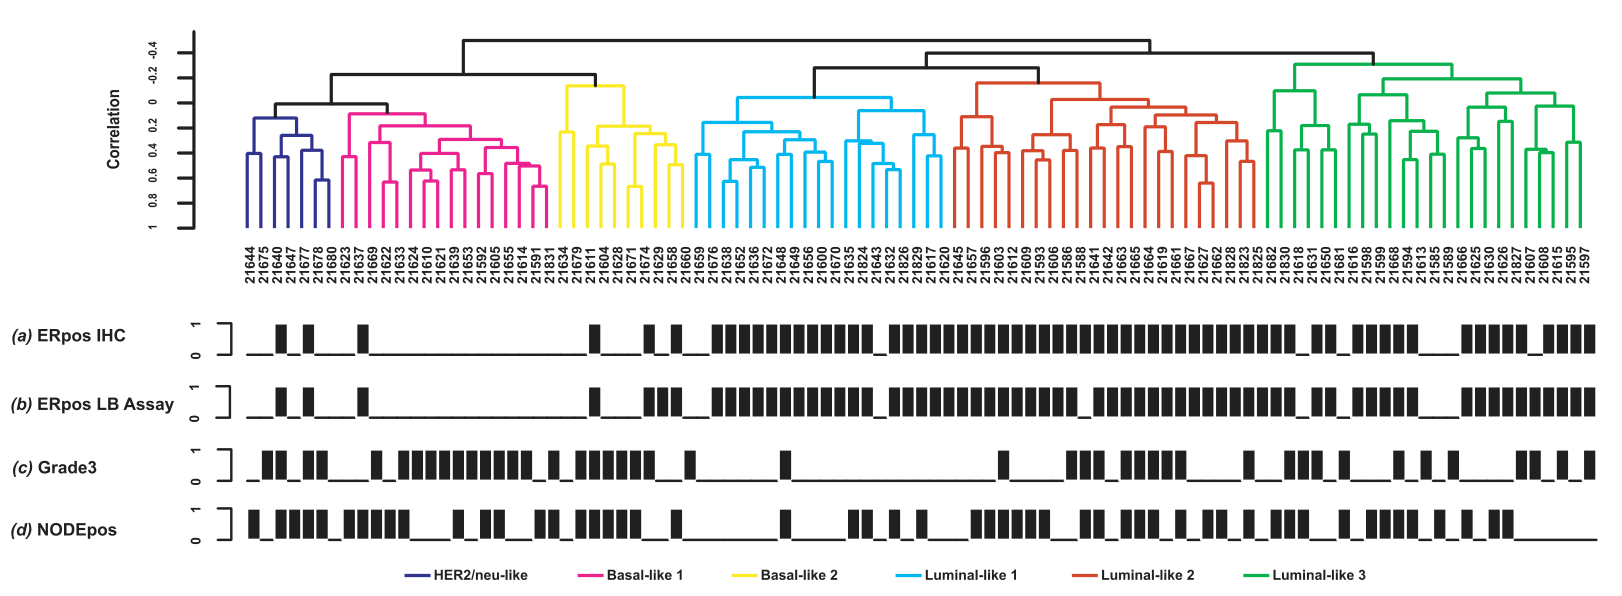
\includegraphics[scale=0.4]{graphics/clustering-in-medicine.png}
	\caption{A hierarchical figure taken from \cite{BreastCancer}. The clusters are seen with the different colours.}
	\label{fig:clustering-genes}
\end{figure}

Clustering is also one of the first steps in machine learning---an example of
unsupervised learning. This just means that the machine ``learns'' of patterns
and structures from the unlabeled data. Sometimes data are put into clusters,
and then nearly all of the data, except for the cluster ID is discarded, which
can save significant space in the analysis stage. To quote Google \cite{Google}:

\begin{displayquote}
	At Google, clustering is used for generalization, data compression, and
	privacy preservation in products such as YouTube videos, Play apps, and
	Music tracks.
\end{displayquote}

There is no one clustering algorithm that is optimal in every situation; in
fact, because data can cluster in many different ways, one needs a whole
clustering toolkit. We will talk about two common methods for clustering:
\textit{$k$-means} and \textit{single linkage} clustering. At the core of both
of these clustering algorithms is a different assumption on the definition of a
cluster. 

\subsection{Introduction to $k$-means clustering}

The idea around $k$-means clustering is incredibly simple: group the data into
$k$ clusters based on the shortest distance to the center of the cluster. From
this, we see how ``cluster'' is interpreted in the $k$-means algorithm---a
cluster forms a ``cell'' in Euclidean space and data points outside of this cell
are outside of the cluster. The shape of these cells depend on the layout of the
centers of the clusters. 

Before we go through the algorithm for $k$-means clustering, let's explore some
of the many applications of this algorithm. 

\subsection{Image compression with $k$-means}

Suppose we have a \texttt{jpg} file that is $m\times n$ pixels. We can turn this
image file into a $3$-dimensional array, namely an $m\times n\times 3$ array.
Alternatively, we can interpret this as three $m\times n$ matrices corresponding
to the red, green, and blue values of the image. 

\begin{wrapfigure}{r}{6cm}
	\centering
	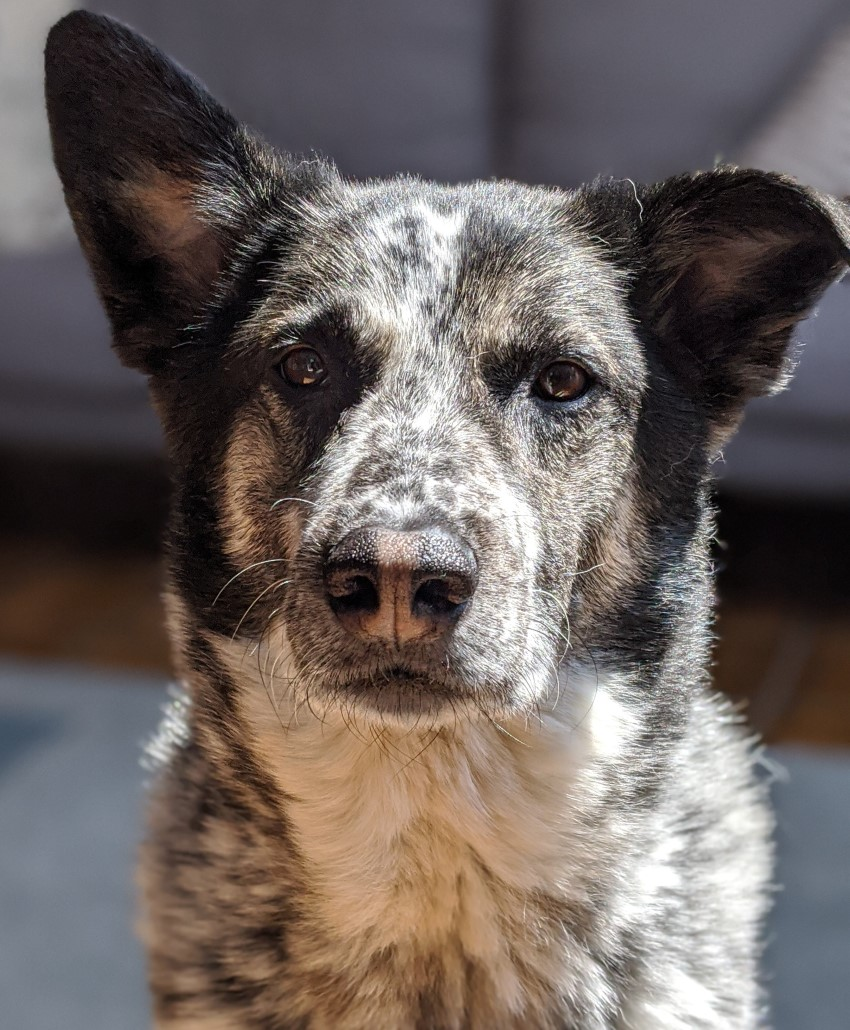
\includegraphics[scale=0.20]{graphics/Sherlock.jpg}
	\caption{Sherlock.}
	\label{fig:sherlock}
\end{wrapfigure}
We can use $k$-means clustering by interpreting each pixel as a data point in
$\R^3$ and determining clusters. Once we find our clusters, we can replace all
the pixels with the center it is closest to. The impact is that we replace all
the different colours with exactly $k$ colours---essentially compressing the
image. 

Let's see how this might look on one of my photos. Meet my dog, Sherlock; he is
depicted in \Cref{fig:sherlock}. There is not very many colours in the image, so
we should expect that low values of $k$ will produce an image that looks fairly
similar. Running a $k$-means clustering for each $k\in \{2,\dots, 10\}$ yields
nine different images seen in \Cref{fig:k-means-sherlock}.

\begin{figure}[h]
	\centering
	% \vspace{-2em}
	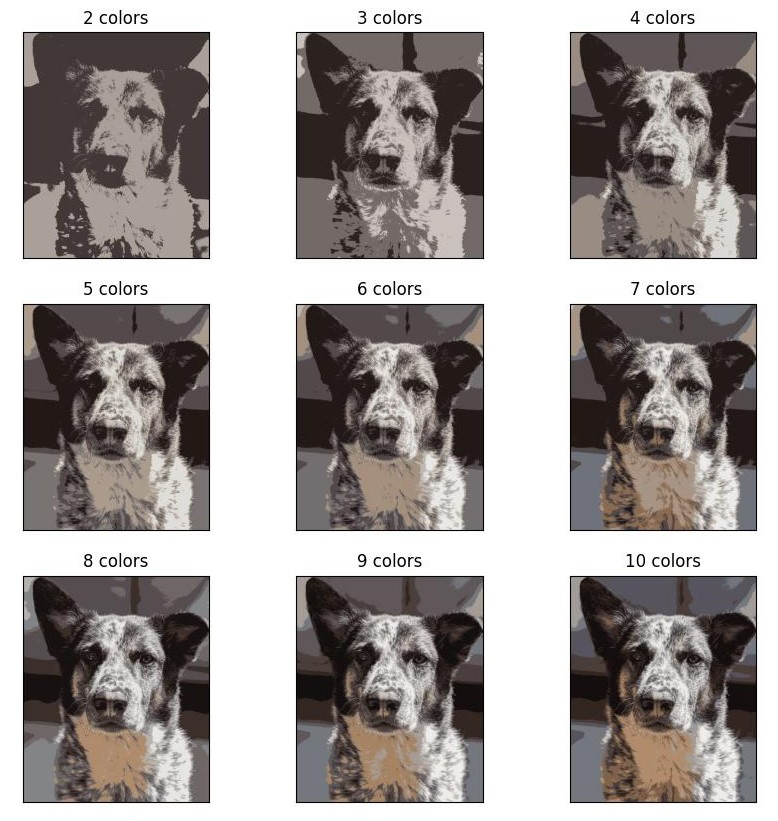
\includegraphics[scale=0.75]{graphics/k_means_Sherlocks.jpg}
	\caption{$k$-means clustering on the image in \Cref{fig:sherlock}.}
	\label{fig:k-means-sherlock}
\end{figure}

\subsection{The $k$-means algorithm}

There are many versions of the basic algorithm we will describe. We use
pseudo-code to give the details of the algorithm; this is a way of giving the
idea of the structure of the code without diving into the specifics of any
particular language. 

We provide pseudo-code for a basic $k$-means algorithm in \Cref{alg:k-means}.
The algorithm returns a function $\Lambda : \{1,\dots, n\} \to \{1,\dots, k\}$,
which can be interpreted as a label for the $n$ data points. The algorithm
accomplishes this by randomly choosing the $k$ centroids, and then clustering
the data points accordingly. Once all the data points have been labeled, we
recompute the centroids by taking the mean point of all the data points in a
given cluster to be the new centroid. 

\begin{algorithm}
	\caption{(Basic) $k$-means}\label{alg:k-means}
	\begin{algorithmic}[1]
		\Require a positive integer $k$ and $n$ data points $x_i\in\R^m$,
		\Ensure a map $\Lambda : \{1,\dots,n\} \to \{1,\dots, k\}$.
		\State Randomly assign the $k$ centroids $c_i$ to $k$ data points.
		\State Let $\Lambda_0$ and $\Lambda$ be constant functions mapping to $-1$ and $0$, respectively.
		\While{$\Lambda_0 \neq \Lambda$}
			\State Set $\Lambda_0 = \Lambda$.
			\For{$i\in \{1,\dots,n\}$}
				\State Set $\Lambda(i) = j$ if $\|x_i-c_j\| = \min\{\|x_i-c_r\| : 1\leq r \leq k\}$.
			\EndFor
			\For{$i\in \{1,\dots, k\}$}
				\State Set $c_i = \left(\sum_{j \in \Lambda^{-1}(i)} x_j\middle) \right/ \# \left(\Lambda^{-1}(i)\right)$.
			\EndFor
		\EndWhile
		\State \Return $\Lambda$.
	\end{algorithmic}
\end{algorithm}

In the first step of $k$-means (see line 1 in \Cref{alg:k-means}), we randomly
assign the $k$ centroids. For different initial assignments, one can get
different outputs. This is like trying to find global extrema on a ``bumpy''
graph by starting at a random point on the graph and then looking for the
nearest local extrema. There are a number of ways to improve the $k$-means
algorithm, we will not cover them, but many consider different variations for
their specific data at hand. 

\subsection{A small example with $k$-means}

We will consider 40 points in $\R^2$, which can be seen in \Cref{fig:4-means},
and we will look for $4$ clusters. You might try to see how you would cluster
the data. 

\begin{figure}[h]
	\centering 
	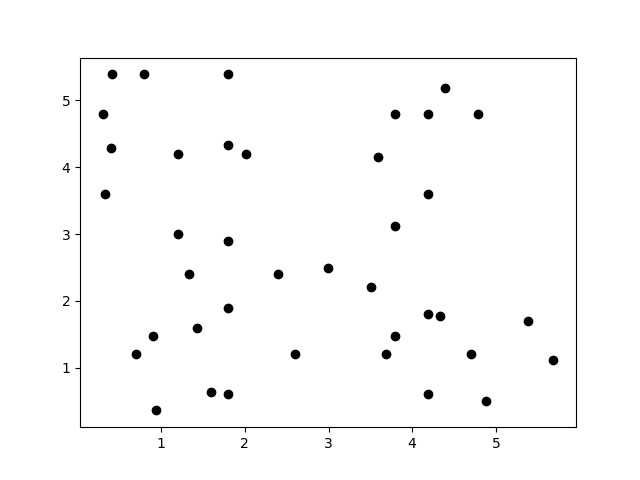
\includegraphics[scale=0.6]{graphics/k_means_iter-1.png}
	\caption{The plotted data we will use to run a $4$-means clustering.}
	\label{fig:4-means}
\end{figure}

We will randomly select four data points for our initial centroids, and then we
will group the data points into the four clusters. We will show this by
colouring the Voronoi cells different colours and indicating the centroids by
white crosses. All of the iterations of one $k$-means algorithm can be seen in
\Cref{fig:4-means-iterations}. Just to illustrate how sensitive $k$-means is to
the initial choice of centroids, we run the algorithm again in
\Cref{fig:4-means-iterations-alt}.



% \afterpage{\clearpage}

\begin{figure}[ht]
	\centering 
	\begin{subfigure}[b]{0.49\textwidth}
		\centering 
		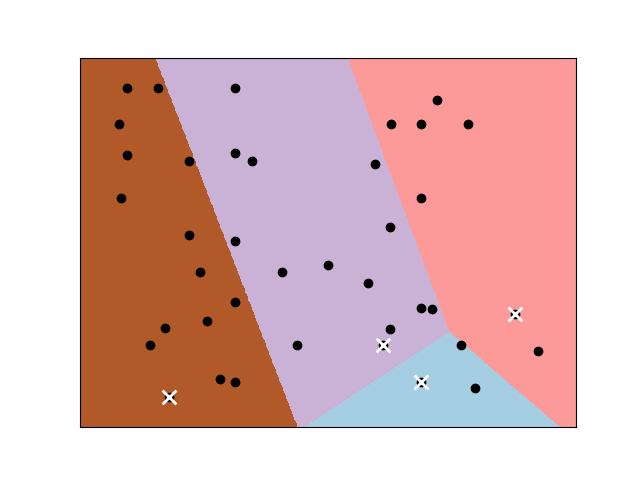
\includegraphics[scale=0.4]{graphics/k_means_iter0.png}
		\vspace{-0.75em}
		\caption{Iteration 0}
	\end{subfigure}~%
	\begin{subfigure}[b]{0.49\textwidth}
		\centering 
		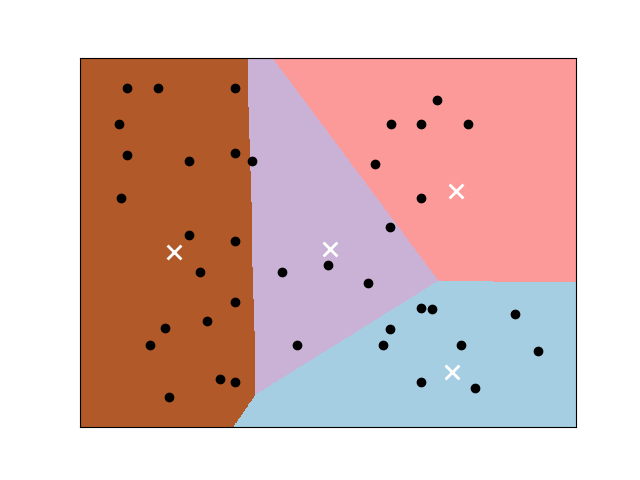
\includegraphics[scale=0.4]{graphics/k_means_iter1.png}
		\vspace{-0.75em}
		\caption{Iteration 1}
	\end{subfigure}
	\begin{subfigure}[b]{0.49\textwidth}
		\centering 
		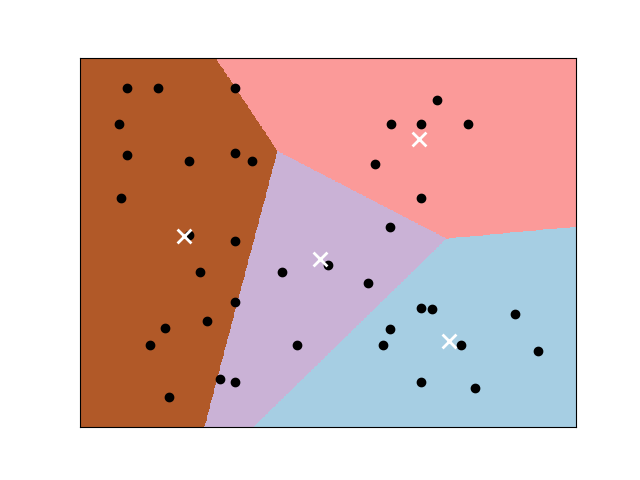
\includegraphics[scale=0.4]{graphics/k_means_iter2.png}
		\vspace{-0.75em}
		\caption{Iteration 2}
	\end{subfigure}~%
	\begin{subfigure}[b]{0.49\textwidth}
		\centering 
		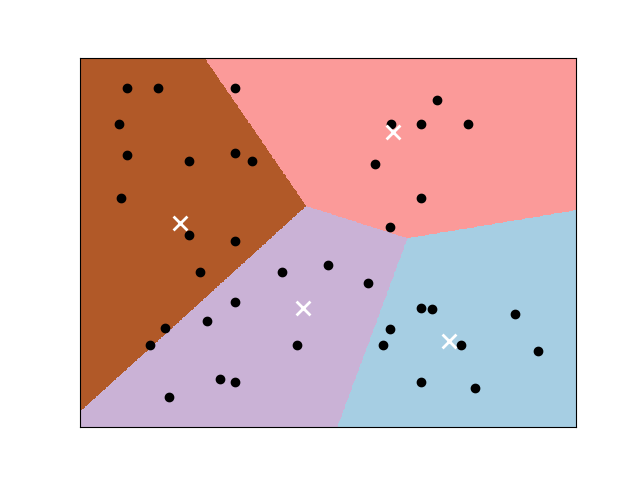
\includegraphics[scale=0.4]{graphics/k_means_iter3.png}
		\vspace{-0.75em}
		\caption{Iteration 3}
	\end{subfigure}
	\begin{subfigure}[b]{0.49\textwidth}
		\centering 
		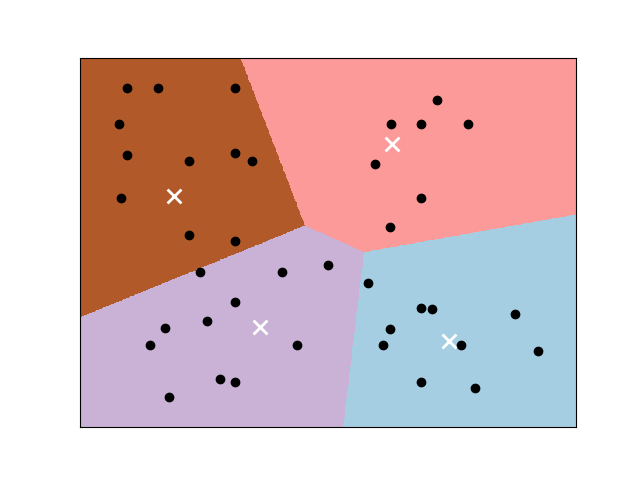
\includegraphics[scale=0.4]{graphics/k_means_iter4.png}
		\vspace{-0.75em}
		\caption{Iteration 4}
	\end{subfigure}~%
	\begin{subfigure}[b]{0.49\textwidth}
		\centering 
		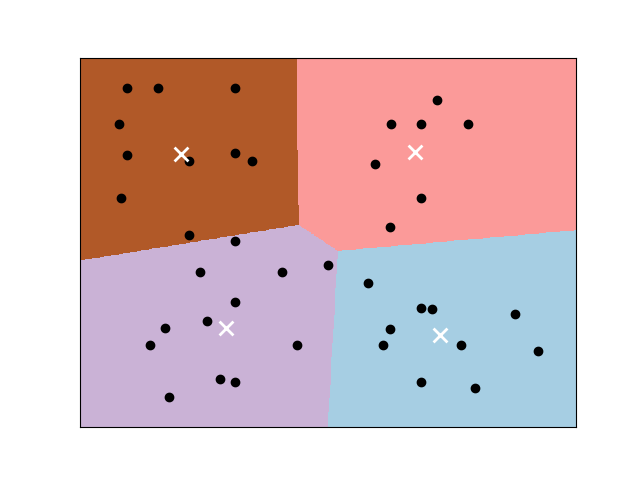
\includegraphics[scale=0.4]{graphics/k_means_iter5.png}
		\vspace{-0.75em}
		\caption{Iteration 5}
	\end{subfigure}
	\begin{subfigure}[b]{0.66\textwidth}
		\centering 
		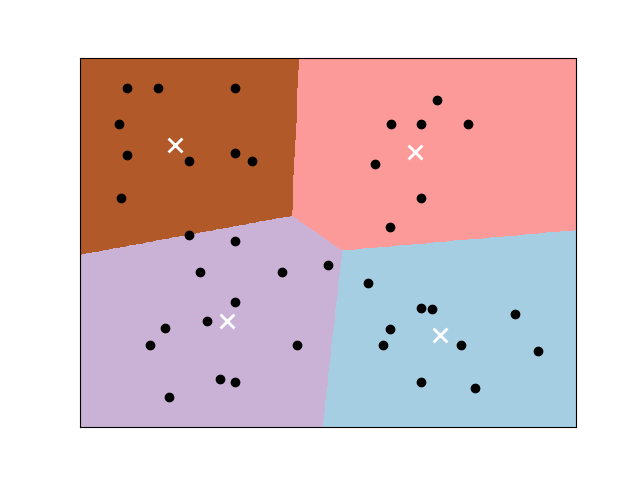
\includegraphics[scale=0.4]{graphics/k_means_iter6.png}
		\vspace{-0.75em}
		\caption{Iteration 6}
	\end{subfigure}
	\caption{Seven iterations of one $k$-means algorithm.}
	\label{fig:4-means-iterations}
\end{figure}

\begin{figure}[t]
	\centering 
	\begin{subfigure}[b]{0.49\textwidth}
		\centering 
		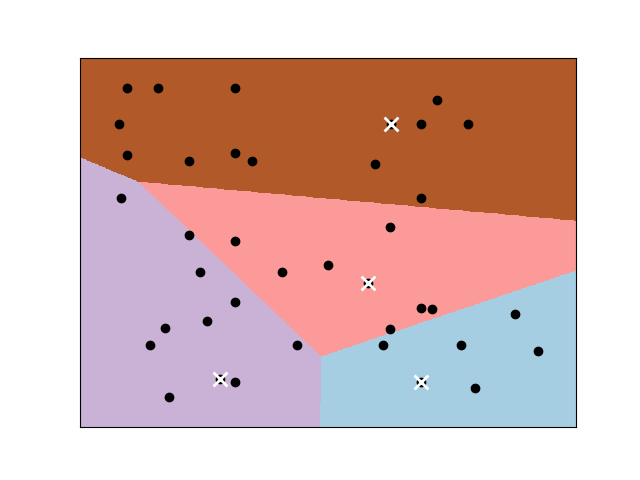
\includegraphics[scale=0.4]{graphics/k_means_iter0_alt.png}
		\vspace{-0.75em}
		\caption{Iteration 0}
	\end{subfigure}~%
	\begin{subfigure}[b]{0.49\textwidth}
		\centering 
		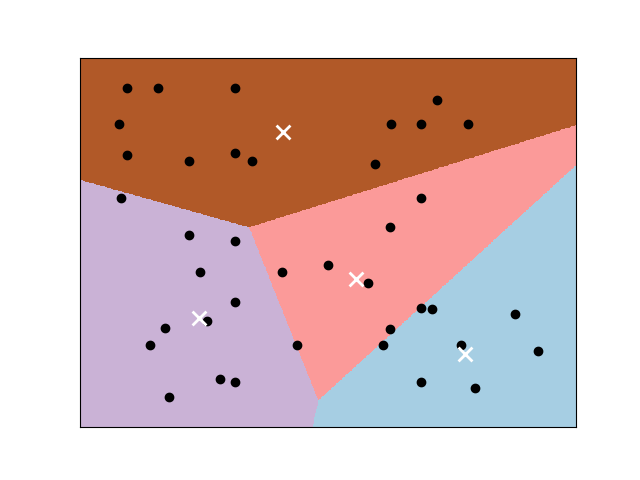
\includegraphics[scale=0.4]{graphics/k_means_iter1_alt.png}
		\vspace{-0.75em}
		\caption{Iteration 1}
	\end{subfigure}
	\begin{subfigure}[b]{0.49\textwidth}
		\centering 
		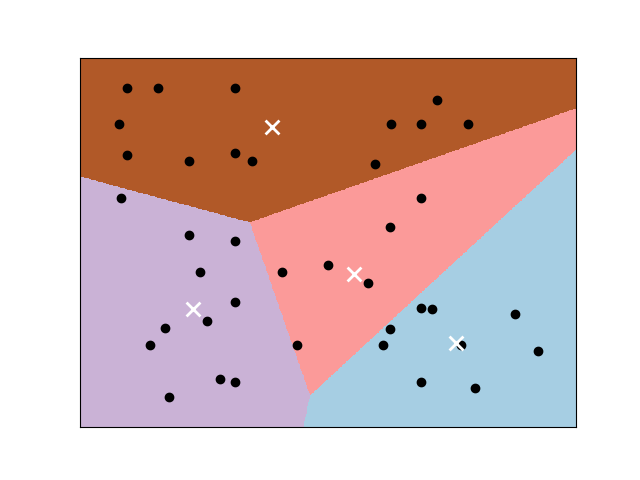
\includegraphics[scale=0.4]{graphics/k_means_iter2_alt.png}
		\vspace{-0.75em}
		\caption{Iteration 2}
	\end{subfigure}~%
	\begin{subfigure}[b]{0.49\textwidth}
		\centering 
		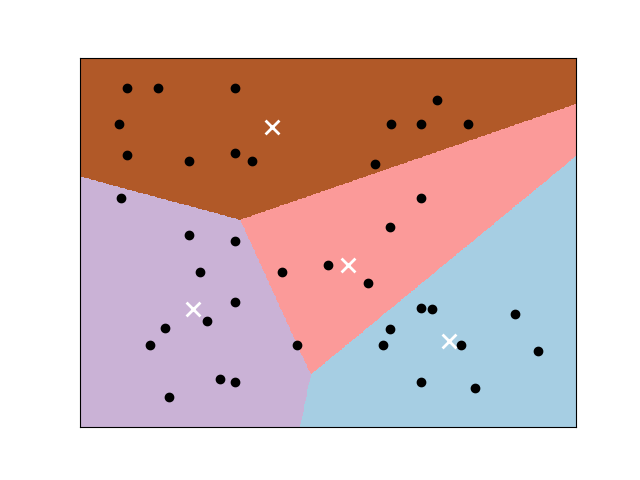
\includegraphics[scale=0.4]{graphics/k_means_iter3_alt.png}
		\vspace{-0.75em}
		\caption{Iteration 3}
	\end{subfigure}
	\caption{Four iterations of another $k$-means algorithm.}
	\label{fig:4-means-iterations-alt}
\end{figure}

\subsection{Introduction to hierarchical clustering}

Hierarchical clustering is, in some sense, the opposite approach to clustering
than $k$-means. We will primarily be working with Single-linkage clustering.
Single-linkage or, more generally, \emph{neighbour joining} clustering is a
hierarchical clustering algorithm. With $k$-means, we need to give the number of
clusters $k$ in order to run the algorithm. With neighbour joining, we look at
all the possible clusterings under prescribed conditions by means of a
\emph{dendrogram}. We have already seen an example of the output of a
hierarchical clustering algorithm; see \Cref{fig:clustering-genes}.

The basic idea of neighbour joining clustering is that every data point is its
own cluster and under certain conditions, two clusters are merged at each step
until all points are in one cluster. The output is not a specific clustering of
the data, but rather all the possible clusterings. This is communicated through
a dendrogram. 

Before we look at the algorithm, let's consider a specific application.

\subsection{An application of hierarchical clustering}

We will look at the study in~\cite{BreastCancer} a little closely; see also
\Cref{fig:clustering-genes}. People diagnosed with breast cancer can have very
different clinical outcomes. We do not really know why this is the case, but one
suggestion might be that our knowledge of the specific breast cancer tumors is
lacking. Sotiriou et al.~\cite{BreastCancer} propose clustering the tumors by
gene expression profiles, via unsupervised hierarchical clustering. 

Prior to their work, the tumors could be partitioned into two major subgroups
based on their estrogen receptors. Using clustering methods, Sotiriou et al.
were able to obtain this partition at the top of the dendrogram---if one cuts it
so there are exactly two clusters, these align with the two subgroups based on
estrogen receptors. They were able to further partition the two subgroups based
on their basal and luminal characteristics. This led to the six clusters
(represented by different colours) in \Cref{fig:clustering-genes}. This is also
in line with previous work done by different research teams, and offers more
evidence that their hypothesis is correct---that breast cancer tumors ought to
be clustered in the established way.

\subsection{The neighbour joining algorithm}

We will describe a class of \emph{agglomerative} algorithms that can be altered
to produce different outcomes based on certain given conditions. In order to do
this, one of the inputs is a distance function, which can be obtained from a
\emph{metric}. We want the metric to be defined on finite subsets of $\R^m$,
which will be interpreted as clusters in the actual algorithm. 

\begin{defn}
	A function $d: \mathscr{M}\times \mathscr{M} \to \R$ on a set $\mathscr{M}$
	is a \emph{metric} if 
	\begin{enumerate}
		\item for all $X, Y\in \mathscr{M}$, we have $d(X, Y) \geq 0$, where
		equality holds if and only if $X=Y$,
		\item for all $X, Y\in\mathscr{M}$, we have $d(X, Y) = d(Y, X)$, and
		\item for all $X, Y, Z\in\mathscr{M}$, the triangle inequality is
		satisfied:
		\[ 
			d(X, Y) + d(Y, Z) \geq d(X, Z). 
		\] 
	\end{enumerate}
	Functions satisfying (1) and (2) are called \emph{semimetrics}. 
\end{defn}

\begin{lem}\label{lem:semimetrics}
	The Euclidean distance $d(x,y) = \|x-y\|$ is a metric on $\R^m$. The square
	of the Euclidean distance, $d_{\square}(x,y)=\|x-y\|^2$, is not a metric but
	a semimetric.
\end{lem}

\begin{proof}
	To show that $d_{\square}$ does not satisfy the triangle inequality, let
	$a\in\R$ be positive. Then $|-a|^2 + |a|^2 < |2a|^2$, so
	\begin{align*}
		d_{\square}(a,0) + d_{\square}(-a,0) &< d_{\square}(a,-a). \qedhere
	\end{align*}
\end{proof}

In the context of clustering, having a metric is not necessary. For example,
because $x\mapsto x^2$ is monotonically increasing on the $\R_{\geq 0}$, it
follows that $d(x,y) < d(u,v)$ if and only if $d_{\square}(x,y) <
d_{\square}(u,v)$; here we are using the notation from \Cref{lem:semimetrics}.
Thus, it is irrelevant if we cluster two points based on $d$ or $d_{\square}$,
so we allow our distance functions to come from semimetrics. 

Let's write $\mathscr{F}_m$ for the set of finite subsets of $\R^m$, so we will
describe a few distance functions on $\mathscr{F}_m$.
\begin{description}
	\item[Single-linkage:] For $C_1,C_2\in\mathscr{F}_m$, 
	\begin{align*}
		d(C_1, C_2) &= \min\left\{ \| x - y\| : x\in C_1, y\in C_2 \right\}. 
	\end{align*}
	\item[Complete-linkage:] For $C_1,C_2\in\mathscr{F}_m$, 
	\begin{align*}
		d(C_1, C_2) &= \max\left\{ \| x - y\| : x\in C_1, y\in C_2 \right\}. 
	\end{align*}
	\item[Average-linkage:] For $C_1,C_2\in\mathscr{F}_m$, 
	\begin{align*}
		d(C_1, C_2) &= \dfrac{1}{\# C_1 \cdot \# C_2} \sum_{x \in C_1} \sum_{y\in C_2} \|x - y\|. 
	\end{align*}
\end{description}
Technically the single-linkage is not a semimetric: if $C_1\cap C_2\neq
\varnothing$ yet $C_1\neq C_2$, then $d(C_1, C_2)=0$. However we only consider
sets $C_1$ and $C_2$ with trivial intersection anyways, so this problem is
avoided. 

\begin{lem}
	The complete-linkage function defines a metric on $\mathscr{F}_m$.
\end{lem}

There are of course other distances one could use. Single-linkage clustering, or
nearest neighbour, corresponds to neighbour joining with the single-linkage
metric. Likewise, complete-linkage clustering, or farthest neighbour,
corresponds to neighbour joining with the complete-linkage metric. One could
design a metric that might be most relevant for the particular data set at hand.

The output for a hierarchical clustering algorithm is a \emph{dendrogram} or
data equivalent to one. \Cref{fig:clustering-genes} contains one example.
Another very similar example is a phylogenetic tree seen in
\Cref{fig:phylogenetic}.

\begin{figure}[h]
	\centering 
	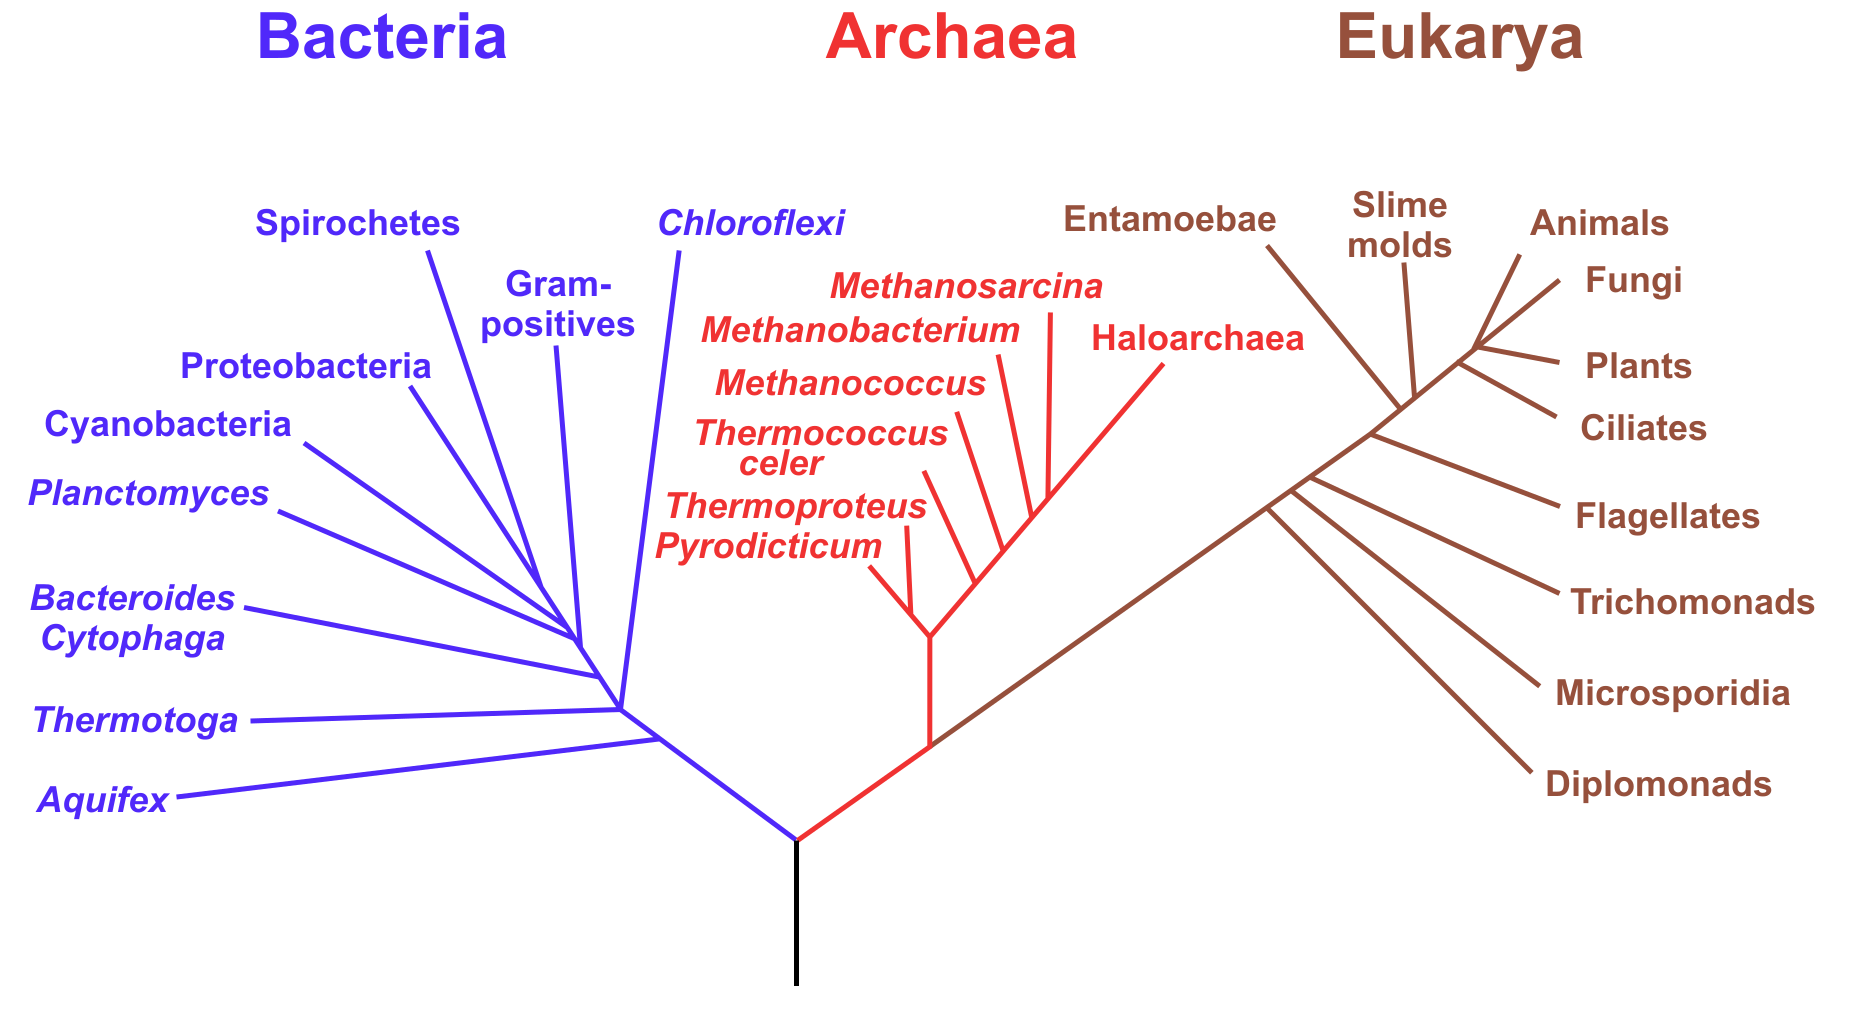
\includegraphics[scale=0.3]{graphics/Phylogenetic_tree.png}
	\caption{A phylogenetic tree is equivalent to a dendrogram.}
	\label{fig:phylogenetic}
\end{figure}

To read a dendrogram, one first finds the many leaves or ends---often these are
labeled---these are the initial clusters. As one goes through the dendrogram
(e.g.\ bottom to top or left to right), clusters get linked, which is depicted
by joining the ends of the initial clusters. This happens until there is exactly
one cluster left. Two ends are closer (or more similar) if they become joined
early on compared to two ends that only become joined near the end of the
dendrogram. 

Let's explain the algorithm using pseudo-code. Instead of outputting a
dendrogram, we will output a list of pairs of the form $(t, [C_1,\dots, C_r])$,
where $t\geq 0$ and each $C_i$ is a finite set of data points. This list will
start with $(0, [C_1,\dots, C_n])$, where each $C_i$ is a singleton, and it will
end with $(t_\infty, [C_1])$, where $C_1$ contains all of the data points. Note
that this data is also equivalent to a dendrogram.

\begin{algorithm}
	\caption{Neighbour joining}\label{alg:neighbour}
	\begin{algorithmic}[1]
		\Require a semimetric $d : \mathscr{F}_m\times \mathscr{F}_m\to \R$ and $n$ data points $x_i\in\R^m$,
		\Ensure a list $D$ equivalent to a dendrogram.
		\State Set $t=0$.
		\State Set $C = \{\{x_1\}, \dots, \{x_n\}\}$.
		\State Set $D = [(t, C)]$.
		\While{$\# C > 1$}
			\State Construct distance matrix $M = (M_{ij})$, with $M_{ij} = d(C_i, C_j)$.
			\State Determine the two closest distinct clusters $C_r$ and $C_s$ from $M$.
			\State Set $t = t + M_{rs}$.
			\State Set $C = (C \setminus \{C_r, C_s\}) \cup \{C_r \cup C_s\}$.
			\State Append to $D$ the pair $(t, C)$.
		\EndWhile
		\State \Return $D$.
	\end{algorithmic}
\end{algorithm}

We will soon go through \Cref{alg:neighbour} on a small example. Unlike
$k$-means, neighbour joining is \emph{deterministic}; that is, it runs the same
every time on the same input. Notice in \Cref{alg:neighbour} that the actual
points $x_i$ do not matter; instead, it's the distances between the points (and
clusters) that matter. Thus, we won't specify points but a \emph{graph}.

\begin{defn}
	A (finite, simple) \textbf{graph} $G$ is a pair of vertices $V = \{v_1,
	\dots, v_n\}$ and edges $E = \{e_1, \dots, e_k\}$, where each $e_i\subseteq
	V$ of size exactly two. Vertices $v_i$ and $v_j$ are \textbf{adjacent},
	written $v_i \sim v_j$, if $\{v_i, v_j\} \in E$.
\end{defn}

Graphs are ubiquitous in mathematics and computer science, and they can be
easily visualised (for a relatively small amount of vertices). Three graphs can
be seen in \Cref{fig:3-graphs}.

\begin{figure}[h]
	\centering
	\begin{minipage}{0.3\textwidth}
		\centering
		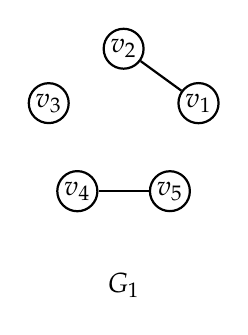
\begin{tikzpicture}
			% Nodes
			\foreach \i in {1,2,3,4,5} {
				\node[circle, draw, fill=white, inner sep=1pt, thick] (node\i) at ({360/5 * (\i - 1) + 18}:1) {$v_{\i}$};
			}
			\node at (0,-2) {$G_1$};
			\draw[thick] (node1) -- (node2);
			\draw[thick] (node4) -- (node5);
		\end{tikzpicture}
	\end{minipage}~
	\begin{minipage}{0.3\textwidth}
		\centering
		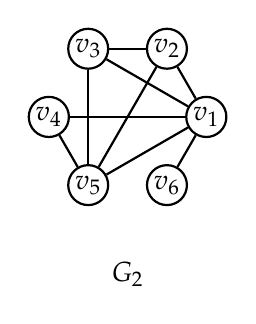
\begin{tikzpicture}
			% Nodes
			\foreach \i in {1,2,3,4,5,6} {
				\node[circle, draw, fill=white, inner sep=1pt, thick] (node\i) at ({360/6 * (\i - 1)}:1) {$v_{\i}$};
			}
			\node at (0,-2) {$G_2$};
			\draw[thick] (node1) -- (node2);
			\draw[thick] (node1) -- (node3);
			\draw[thick] (node1) -- (node4);
			\draw[thick] (node1) -- (node5);
			\draw[thick] (node1) -- (node6);
			\draw[thick] (node2) -- (node3);
			\draw[thick] (node2) -- (node5);
			\draw[thick] (node4) -- (node5);
			\draw[thick] (node3) -- (node5);
		\end{tikzpicture}
	\end{minipage}~
	\begin{minipage}{0.3\textwidth}
		\centering
		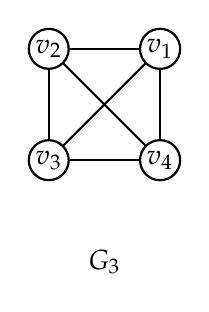
\begin{tikzpicture}
			% Nodes
			\foreach \i in {1,2,3,4} {
				\node[circle, draw, fill=white, inner sep=1pt, thick] (node\i) at ({360/4 * (\i) - 45}:1) {$v_{\i}$};
			}
			\node at (0,-2) {$G_3$};
			\draw[thick] (node1) -- (node2);
			\draw[thick] (node1) -- (node3);
			\draw[thick] (node1) -- (node4);
			\draw[thick] (node2) -- (node3);
			\draw[thick] (node2) -- (node4);
			\draw[thick] (node3) -- (node4);
		\end{tikzpicture}
	\end{minipage}
	\caption{Three different graphs.}
	\label{fig:3-graphs}
\end{figure}

\subsection{A small example of hierarchical clustering}

Instead of writing down or plotting data points, we will write down a distance
matrix. The distance matrix is a symmetric matrix with zeros along the diagonal.
(Why?) The $(i,j)$ entry is equal to the distance between vertices (or clusters)
$v_i$ and $v_j$. Let's consider the following distance matrix.
\begin{center}
	\begin{tabular}{c|cccccc}
		& $v_1$ & $v_2$ & $v_3$ & $v_4$ & $v_5$ & $v_6$ \\ \hline 
		$v_1$ & 0 & 4 & 8 & 1 & 7 & 8 \\
		$v_2$ & 4 & 0 & 6 & 5 & 5 & 6 \\
		$v_3$ & 8 & 6 & 0 & 7 & 2 & 2 \\
		$v_4$ & 1 & 5 & 7 & 0 & 8 & 8 \\
		$v_5$ & 7 & 5 & 2 & 8 & 0 & 1 \\
		$v_6$ & 8 & 6 & 2 & 8 & 1 & 0 
	\end{tabular}
\end{center}

We will apply single- and complete-linkages and cluster the data accordingly.
Because we know how to compute them both given the distances from all pairs of
vertices, we will not recompute our distance matrix each time. Instead we will
draw nine graphs labeled $G_t$ for $t\in \{0, \dots, 8\}$ since the maximal
distance between any two points is $8$. We will include an edge between $v_i$
and $v_j$ in $G_t$ if and only if $d(v_i, v_j)\leq t$. The graph $G_0$ is the
graph on 8 vertices with no edges, and the graph $G_8$ is the graph on 8
vertices where every vertex is adjacent to every other vertex (this is called a
\emph{complete graph}). All of the graphs are shown in \Cref{fig:9-graphs}.

\begin{figure}[h]
	\centering 
	\begin{tikzpicture}
		\node at (0, 2*4) {
		\begin{tikzpicture}
			% Nodes
			\foreach \i in {1,2,3,4,5,6} {
				\node[circle, draw, fill=white, inner sep=1pt, thick] (node\i) at ({360/6 * (\i - 1)}:1) {$v_{\i}$};
			}
			\node at (0, -1.75) {$G_0$};
		\end{tikzpicture}
		};
		\node at (1*4.5, 2*4) {
		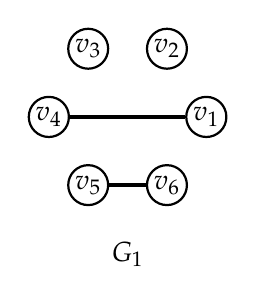
\begin{tikzpicture}
			% Nodes
			\foreach \i in {1,2,3,4,5,6} {
				\node[circle, draw, fill=white, inner sep=1pt, thick] (node\i) at ({360/6 * (\i - 1)}:1) {$v_{\i}$};
			}
			\node at (0, -1.75) {$G_1$};
			\draw[ultra thick] (node1) -- (node4);
			\draw[ultra thick] (node5) -- (node6);
		\end{tikzpicture}
		};
		\node at (2*4.5, 2*4) {
		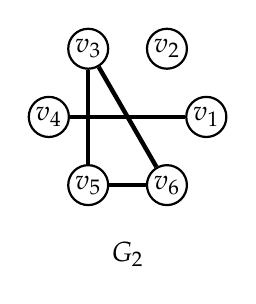
\begin{tikzpicture}
			% Nodes
			\foreach \i in {1,2,3,4,5,6} {
				\node[circle, draw, fill=white, inner sep=1pt, thick] (node\i) at ({360/6 * (\i - 1)}:1) {$v_{\i}$};
			}
			\node at (0, -1.75) {$G_2$};
			\draw[ultra thick] (node1) -- (node4);
			\draw[ultra thick] (node5) -- (node6);
			\draw[ultra thick] (node3) -- (node5);
			\draw[ultra thick] (node3) -- (node6);
		\end{tikzpicture}
		};
		\node at (0, 1*4) {
		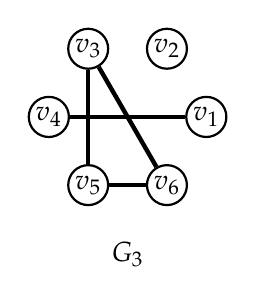
\begin{tikzpicture}
			% Nodes
			\foreach \i in {1,2,3,4,5,6} {
				\node[circle, draw, fill=white, inner sep=1pt, thick] (node\i) at ({360/6 * (\i - 1)}:1) {$v_{\i}$};
			}
			\node at (0, -1.75) {$G_3$};
			\draw[ultra thick] (node1) -- (node4);
			\draw[ultra thick] (node5) -- (node6);
			\draw[ultra thick] (node3) -- (node5);
			\draw[ultra thick] (node3) -- (node6);
		\end{tikzpicture}
		};
		\node at (1*4.5, 1*4) {
		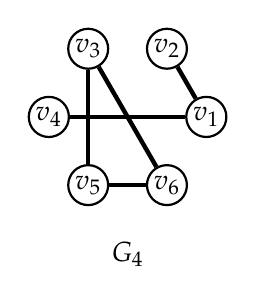
\begin{tikzpicture}
			% Nodes
			\foreach \i in {1,2,3,4,5,6} {
				\node[circle, draw, fill=white, inner sep=1pt, thick] (node\i) at ({360/6 * (\i - 1)}:1) {$v_{\i}$};
			}
			\node at (0, -1.75) {$G_4$};
			\draw[ultra thick] (node1) -- (node4);
			\draw[ultra thick] (node5) -- (node6);
			\draw[ultra thick] (node3) -- (node5);
			\draw[ultra thick] (node3) -- (node6);
			\draw[ultra thick] (node1) -- (node2);
		\end{tikzpicture}
		};
		\node at (2*4.5, 1*4) {
		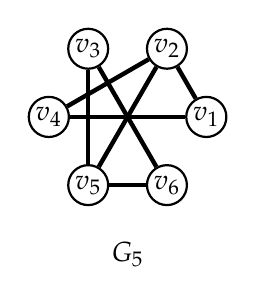
\begin{tikzpicture}
			% Nodes
			\foreach \i in {1,2,3,4,5,6} {
				\node[circle, draw, fill=white, inner sep=1pt, thick] (node\i) at ({360/6 * (\i - 1)}:1) {$v_{\i}$};
			}
			\node at (0, -1.75) {$G_5$};
			\draw[ultra thick] (node1) -- (node4);
			\draw[ultra thick] (node5) -- (node6);
			\draw[ultra thick] (node3) -- (node5);
			\draw[ultra thick] (node3) -- (node6);
			\draw[ultra thick] (node1) -- (node2);
			\draw[ultra thick] (node2) -- (node4);
			\draw[ultra thick] (node2) -- (node5);
		\end{tikzpicture}
		};
		\node at (0*4.5, 0) {
		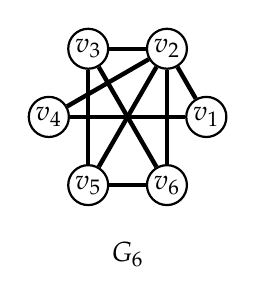
\begin{tikzpicture}
			% Nodes
			\foreach \i in {1,2,3,4,5,6} {
				\node[circle, draw, fill=white, inner sep=1pt, thick] (node\i) at ({360/6 * (\i - 1)}:1) {$v_{\i}$};
			}
			\node at (0, -1.75) {$G_6$};
			\draw[ultra thick] (node1) -- (node4);
			\draw[ultra thick] (node5) -- (node6);
			\draw[ultra thick] (node3) -- (node5);
			\draw[ultra thick] (node3) -- (node6);
			\draw[ultra thick] (node1) -- (node2);
			\draw[ultra thick] (node2) -- (node4);
			\draw[ultra thick] (node2) -- (node5);
			\draw[ultra thick] (node2) -- (node3);
			\draw[ultra thick] (node2) -- (node6);
		\end{tikzpicture}
		};
		\node at (1*4.5, 0) {
		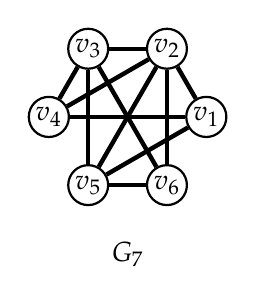
\begin{tikzpicture}
			% Nodes
			\foreach \i in {1,2,3,4,5,6} {
				\node[circle, draw, fill=white, inner sep=1pt, thick] (node\i) at ({360/6 * (\i - 1)}:1) {$v_{\i}$};
			}
			\node at (0, -1.75) {$G_7$};
			\draw[ultra thick] (node1) -- (node4);
			\draw[ultra thick] (node5) -- (node6);
			\draw[ultra thick] (node3) -- (node5);
			\draw[ultra thick] (node3) -- (node6);
			\draw[ultra thick] (node1) -- (node2);
			\draw[ultra thick] (node2) -- (node4);
			\draw[ultra thick] (node2) -- (node5);
			\draw[ultra thick] (node2) -- (node3);
			\draw[ultra thick] (node2) -- (node6);
			\draw[ultra thick] (node1) -- (node5);
			\draw[ultra thick] (node3) -- (node4);
		\end{tikzpicture}
		};
		\node at (2*4.5, 0) {
		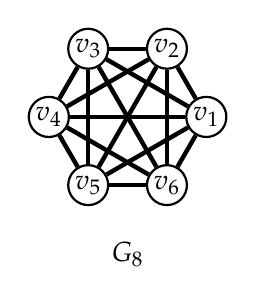
\begin{tikzpicture}
			% Nodes
			\foreach \i in {1,2,3,4,5,6} {
				\node[circle, draw, fill=white, inner sep=1pt, thick] (node\i) at ({360/6 * (\i - 1)}:1) {$v_{\i}$};
			}
			\node at (0, -1.75) {$G_8$};
			\draw[ultra thick] (node1) -- (node4);
			\draw[ultra thick] (node5) -- (node6);
			\draw[ultra thick] (node3) -- (node5);
			\draw[ultra thick] (node3) -- (node6);
			\draw[ultra thick] (node1) -- (node2);
			\draw[ultra thick] (node2) -- (node4);
			\draw[ultra thick] (node2) -- (node5);
			\draw[ultra thick] (node2) -- (node3);
			\draw[ultra thick] (node2) -- (node6);
			\draw[ultra thick] (node1) -- (node5);
			\draw[ultra thick] (node3) -- (node4);
			\draw[ultra thick] (node1) -- (node3);
			\draw[ultra thick] (node1) -- (node6);
			\draw[ultra thick] (node4) -- (node5);
			\draw[ultra thick] (node4) -- (node6);
		\end{tikzpicture}
		};
	\end{tikzpicture}
	\caption{The 9 graphs visualising the possible clustering of the 8 vertices.}
	\label{fig:9-graphs}
\end{figure}


Now we will produce dendrograms, one for the single-linkage and one for the
complete-linkage. There are two concepts in Graph Theory that we can use to
determine these dendrograms. 

\begin{defn}
	Two vertices $v_i$ and $v_j$ of a graph $G$ are \textbf{connected} if there
	exists a sequence of adjacent vertices of the form $v_i = v_0 ~ v_1 ~ \cdots
	~ v_{\ell} = v_j$.
\end{defn}

\begin{defn}
	A subset $S$ of vertices of a graph $G$ form a \textbf{clique} if for all
	distinct $v_i, v_j\in S$, the edge $\{v_i, v_j\}$ is in $G$. 
\end{defn}

Let's consider the graphs in \Cref{fig:9-graphs} again. Using single-linkage, we
know that vertices $v_i$ and $v_j$ lie in the same cluster if and only if $v_i$
and $v_j$ are connected. Therefore, we have exactly one cluster starting at
$G_5$ using single-linkage. Using complete-linkage, we know that vertices
$\{v_{i_1}, \dots, v_{i_{\ell}}\}$ form a cluster if and only if they form a
clique. Hence, we have exactly one cluster starting at $G_8$ using
complete-linkage. The dendrograms can be seen in
\Cref{fig:dendrogram-slink,,fig:dendrogram-clink}. 

% \afterpage{\clearpage}

\begin{figure}[h]
	\centering 
	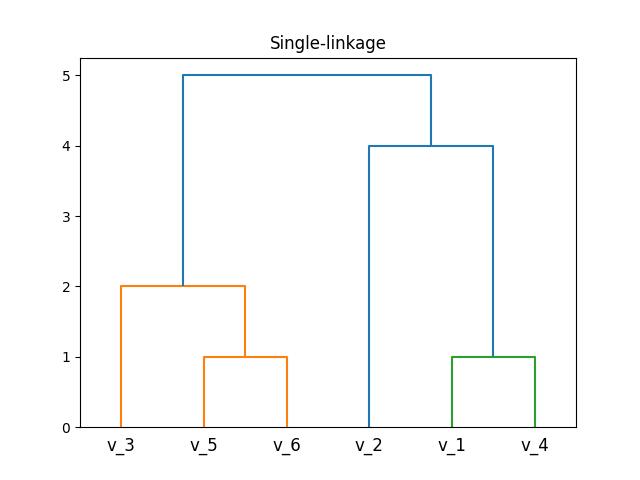
\includegraphics[scale=0.75]{graphics/slink.png}
	\caption{The dendrogram corresponding to the graphs in \Cref{fig:9-graphs} using single-linkage.}
	\label{fig:dendrogram-slink}	
\end{figure}

\begin{figure}[h]
	\centering 
	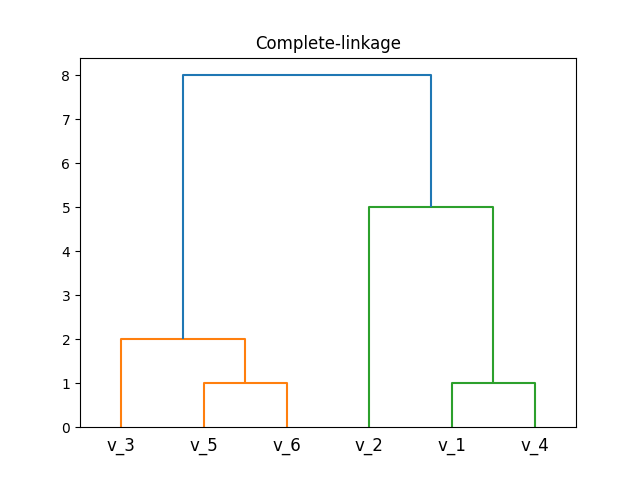
\includegraphics[scale=0.75]{graphics/clink.png}
	\caption{The dendrogram corresponding to the graphs in \Cref{fig:9-graphs} using complete-linkage.}
	\label{fig:dendrogram-clink}	
\end{figure}

































\newpage

\begin{bibdiv}
\begin{biblist}
	\bib{BreastCancer}{article}{
		title={Breast cancer classification and prognosis based on gene expression profiles from a population-based study},
		author={Sotiriou, Christos},
		author={Neo, Soek-Ying},
		author={McShane, Lisa M.},
		author={Korn, Edward L.},
		author={Long, Philip M.},
		author={Jazaeri, Amir},
		author={Martiat, Philippe},
		author={Fox, Steve B.},
		author={Harris, Adrian L.},
		author={Liu, Edison T.},
		journal={Proceedings of the National Academy of Sciences},
		volume={100},
		number={18},
		pages={10393--10398},
		year={2003},
		publisher={National Acad Sciences},
	}

	\bib{FM/90}{article}{
		author={Frankl, Peter},
		author={Maehara, Hiroshi},
		title={Some geometric applications of the beta distribution},
		journal={Ann. Inst. Statist. Math.},
		volume={42},
		date={1990},
		number={3},
		pages={463--474},
		issn={0020-3157},
	}

	\bib{Google}{article}{
		author={Google},
		title={What is Clustering?}
		date={2023},
		status={date accessed: 16 Oct.\ 2023. \url{https://developers.google.com/machine-learning/clustering/overview}},
	}

	\bib{HPIM/12}{article}{
		author={Har-Peled, Sariel},
		author={Indyk, Piotr},
		author={Motwani, Rajeev},
		title={Approximate nearest neighbor: towards removing the curse of
		dimensionality},
		journal={Theory Comput.},
		volume={8},
		date={2012},
		pages={321--350},
		review={\MR{2948494}},
		doi={10.4086/toc.2012.v008a014},
	}

	\bib{ILA}{book}{
		author={Margalit, Dan},
		author={Rabinoff, Joseph},
		title={Interactive Linear Algebra},
		date={2019},
		status={\url{https://textbooks.math.gatech.edu/ila/}},
	}

	\bib{Shlens}{unpublished}{
		author={Shlens, Jonathon},
		title={A tutorial on principal component analysis},
		date={2014},
		status={\href{https://arxiv.org/abs/1404.1100}{\texttt{arXiv:1404.1100}}},
	}

	\bib{YLDW/21}{unpublished}{
      title={How to reduce dimension with PCA and random projections?}, 
      author={Fan Yang and Sifan Liu and Edgar Dobriban and David P. Woodruff},
      year={2021},
      status={\href{https://arxiv.org/abs/2005.00511}{\texttt{arXiv:2005.00511}}}, 
	}
\end{biblist}
\end{bibdiv}

\end{document}